\documentclass[UdineBachThesis,american,11pt,draft]{PhdThesis}

\usepackage{babel}
\usepackage[final]{graphicx}

\usepackage{amsmath}
\usepackage{amssymb}

\usepackage{csquotes}
\usepackage{enumitem}
\usepackage[final]{listings}
\usepackage{multirow}

\usepackage{biblatex}
\addbibresource{thesis.bib}

\usepackage{tikz}
\usetikzlibrary{positioning}
\usetikzlibrary{shapes.geometric}

\usepackage{theorems}

\author{Matteo Morena}
\supervisor{Prof.\ Marco Comini}
\date{2022--2023}

\title{
  Implementation of an interpreter with graphical interface of a simple
  imperative language
}

\setlength{\evensidemargin}{3mm}
\setlength{\oddsidemargin}{7mm}
\setlength{\textwidth}{150mm}
\setlength{\parindent}{0pt}
\setlength{\parskip}{0.4em plus 1pt minus 1pt}

\setlist{
  topsep=0pt,
  partopsep=0pt,
  parsep=\parskip,
  itemsep=0pt
}

\lstset{
  aboveskip=\parskip,
  belowskip=0pt,
  basicstyle=\ttfamily,
  upquote=true,
  captionpos=b,
  abovecaptionskip=\abovecaptionskip,
  belowcaptionskip=\belowcaptionskip,
  columns=fullflexible,
  keepspaces=true,
  literate={‘}{`}{1}{’}{'}{1}{“}{`}{1}{”}{'}{1},
  frame=single
}

\begin{document}
  \pagestyle{empty}

  \maketitle

  \begin{abstract}
    % TODO
  \end{abstract}

  \begin{acknowledgments}
    % TODO
  \end{acknowledgments}

  \frontmatter

  \tableofcontents

  \mainmatter

  \pagestyle{serif}
  \partstyle{serifbig}
  \chaptertitlestyle{serifbig}

  \chapter{Haskell programming}

  This chapter gives an overview of the Haskell programming language. I'll
  assume the reader is familiar with any imperative programming language like C,
  C++ or Java.

  Haskell is a purely functional programming language. Programs are not encoded
  as a series of steps and procedures abstracting over them; in particular,
  there is no such thing as a statement. Instead, everything in Haskell is an
  expression; functions are the building blocks which abstract over expressions.

  Functions operate on their arguments and compute some result; if a function
  gets called twice with the same arguments, it's guaranteed to yield the same
  result: this is called \emph{referential transparency}. This property
  guarantees that every function application can be substituted with its
  corresponding value; thinking about execution as such a rewrite system can
  improve correctness while making it easier to reason about program behavior.

  In Haskell, expressions are evaluated \emph{lazily} by default; what this
  means is that their value is not computed until it is actually needed. Among
  others, lazy evaluation allows to define and work on infinite data structures
  such as the list of all primes. This evaluation model implies that the order
  of execution isn't defined by the programmer; rather, it is up to the runtime
  to decide when to evaluate what. This goes well with referential transparency
  and it allows to think of programs as a series of transformations on data.

  \section{Expressions and function definitions}

  In Haskell, a program is a set of functions. For instance, the function for
  calculating the hypotenuse of a triangle with catheti \lstinline@x@ and
  \lstinline@y@ can be defined as follows:

  \begin{lstlisting}[gobble=4,basicstyle=\ttfamily\small]
    pythagoras = \x y -> sqrt (x ^ 2  + y ^ 2)
  \end{lstlisting}

  This declaration binds the name \lstinline@pythagoras@ to a function of two
  arguments which applies Pythagoras' theorem. The symbol \lstinline@\@ is
  pronounced \emph{lambda}, as the notation recalls the one used in lambda
  calculus: $\lambda x y . \sqrt{x^2 + y^2}$.

  In Haskell, functions are first-class citizens: they can be used like ordinary
  values. The syntax used earlier makes this explicit, as \lstinline@pythagoras@
  is bound to a value which \emph{is} a function. Alternatively, syntactic sugar
  allows for an equivalent definition:

  \begin{lstlisting}[gobble=4,basicstyle=\ttfamily\small]
    pythagoras x y = sqrt (x ^ 2 + y ^ 2)
  \end{lstlisting}

  Haskell is a \emph{statically typed}. In the definition for
  \lstinline@pythagoras@, \lstinline@x@ and \lstinline@y@ must support
  multiplication, addition and exponentiation; thus, the compiler infers that
  they must be floating-point numbers. Explicit type annotations can be
  provided: in fact, top level definitions conventionally include them for
  clarity:

  \begin{lstlisting}[gobble=4,basicstyle=\ttfamily\small]
    pythagoras :: Floating a => a -> a -> a
    pythagoras x y = sqrt (x ^ 2 + y ^ 2)
  \end{lstlisting}

  The type annotation specifies that, given any type \lstinline@a@ which
  supports floating-point arithmetic, \lstinline@pythagoras@ is a function
  \lstinline@a -> a -> a@. The parameter types are separated with
  \lstinline@(->)@ and there appears to be no special distinction between
  parameter and return types.

  Data in Haskell is immutable; this includes arguments and local bindings.
  Think of implementing a function computing the factorial of a number $n$ in an
  imperative language: probably, you'd have some accumulator initially set to
  $1$ and a loop repeatedly multiplying said accumulator with the numbers from
  $1$ to $n$. As there is no concept of mutable variables in Haskell, other
  mechanisms have to be employed instead; the simplest purely functional
  implementation may use linear recursion:

  \begin{lstlisting}[gobble=4,basicstyle=\ttfamily\small]
    factorial :: Integral a => a -> a
    factorial 0 = 1
    factorial n | n > 0 = n * factorial (n - 1)
  \end{lstlisting}

  The definition above may be read as follows: the factorial of \lstinline@n@ is
  \lstinline@1@ if \lstinline@n@ is \lstinline@0@, and is
  \lstinline@n * factorial (n - 1)@ if \lstinline@n > 0@. The boolean expression
  \lstinline@n > 0@ is called a \emph{guard}, and the result of
  \lstinline@factorial@ is undefined if \lstinline@n < 0@. An equivalent
  definition could have been provided with conditionals:

  \begin{lstlisting}[gobble=4,basicstyle=\ttfamily\small]
    factorial :: Integral a => a -> a
    factorial n =
      if n == 0 then 1
      else if n > 0 then n * factorial (n - 1)
      else undefined
  \end{lstlisting}

  Yet another alternative to define the factorial function is to employ tail
  recursion:

  \begin{lstlisting}[gobble=4,basicstyle=\ttfamily\small]
    factorial' :: Integral a => a -> a
    factorial' n = go 1 n
      where
        go acc 0 = acc
        go acc i | i > 0 = go (acc * i) (i - 1)
  \end{lstlisting}

  The function \lstinline@factorial'@ (the single quote \lstinline@'@ is part of
  its name) employs a local helper function \lstinline@go@ which performs the
  actual computation. Notice that \lstinline@go@ resembles the imperative loop
  from \lstinline@1@ to \lstinline@n@ which accumulates the product into
  \lstinline@acc@. Since Haskell is lazily evaluated, the difference in
  performance between \lstinline@factorial@ and \lstinline@factorial'@ is
  negligible.

  Haskell supports the definition of arbitrary infix operators. For instance,
  an integer exponentiation operator could be defined as follows:

  \begin{lstlisting}[gobble=4,basicstyle=\ttfamily\small]
    (^) :: (Num a, Integral b) => a -> b -> a
    b ^ 0 = 1
    b ^ n | n > 0 = b * (b ^ (n - 1))
  \end{lstlisting}

  Binary infix operators are just functions with a name made up of one or more
  special characters like \lstinline@!@, \lstinline@#@, \lstinline@$@,
  \lstinline@%@, \lstinline@&@, \lstinline@*@, \lstinline@+@, \lstinline@.@,
  \lstinline@/@, \lstinline@<@, \lstinline@=@, \lstinline@>@, \lstinline@?@,
  \lstinline|@|, \lstinline@\@, \lstinline@^@, \lstinline@|@, \lstinline@-@,
  \lstinline@~@, \lstinline@:@. In fact, given \lstinline@b@ and \lstinline@n@,
  the expression \lstinline@b ^ n@ has an equivalent prefix form,
  \lstinline@(^) b n@; a non-symbolic alias can be defined as
  \lstinline@pow = (^)@, making \lstinline@b ^ n@ equivalent to
  \lstinline@pow b n@. Symmetrically, any binary function can be used as an
  infix operator: given the function \lstinline@div@ for integer division
  towards negative infinity, \lstinline@div n d@ has an equivalent infix form,
  \lstinline@n `div` d@.

  \section{Fundamental data types}

  Without importing other modules, Haskell supports the following numeric types:

  \begin{itemize}
    \item \lstinline@Int@: fixed-precision integers at least in the range
    $\left[-2^{29}, 2^{29} - 1\right]$;

    \item \lstinline@Word@: unsigned fixed-precision integers, with the same
    size as \lstinline@Int@.

    \item \lstinline@Integer@: arbitrary precision integers;

    \item \lstinline@Float@: single-precision floating-point numbers;

    \item \lstinline@Double@: double-precision floating-point numbers;

    \item \lstinline@Rational@: rational numbers, represented as a ratio of two
    \lstinline@Integer@ values.
  \end{itemize}

  All numeric types support addition, subtraction, multiplication and
  comparison. The sign of a number \lstinline@x@ can be extracted with
  \lstinline@signum x@; its absolute value can be computed with
  \lstinline@abs x@. The integral data types \lstinline@Int@, \lstinline@Word@
  and \lstinline@Integer@ support integer division towards negative infinity via
  \lstinline@div@ and remainder via \lstinline@mod@. Two numbers \lstinline@x@
  and \lstinline@y@ of the same fractional type can be divided with
  \lstinline@x / y@. Further, many trigonometric, hyperbolic and related
  functions like \lstinline@sin@, \lstinline@cos@, \lstinline@sqt@ and
  \lstinline@log@ are supported by the floating-point data types
  \lstinline@Float@ and \lstinline@Double@. More functions can be found in
  Haskell's standard library; most of them are described in the documentation.

  Besides numeric types, Haskell provides \lstinline@Bool@ and \lstinline@Char@
  as basic data types. These represent the boolean values
  \lstinline@True@/\lstinline@False@ and Unicode scalar values respectively.

  \section{Tuples}

  Multiple values can be grouped into \emph{tuples}. For example,
  two-dimensional vectors $\left(x, y\right)$ can be stored as a 2-tuple of type
  \lstinline@(Double, Double)@; addition, dot product and magnitude functions
  can thus be defined as follows:

  \begin{lstlisting}[gobble=4,basicstyle=\ttfamily\small]
    type Vector2D = (Double, Double)

    sum2D :: Vector2D -> Vector2D -> Vector2D
    sum2D (x1, y1) (x2, y2) = (x1 + x2, y1 + y2)

    dot2D :: Vector2D -> Vector2D -> Double
    dot2D (x1, y1) (x2, y2) = x1 * x2 + y1 * y2

    magnitude2D :: Vector2D -> Double
    magnitude2D v = sqrt (dot2D v v)
  \end{lstlisting}

  The functions \lstinline@sum2D@ and \lstinline@dot2D@ both deconstruct the
  arguments via \emph{pattern matching}: the individual components of the tuples
  are bound to names to be used inside the function definitions. As we'll see,
  pattern matching is extensively used in Haskell.

  For 2-tuples, Haskell provides the \lstinline@fst@ and \lstinline@snd@
  functions to extract the first and second item respectively. Using these,
  \lstinline@sum2D@ and \lstinline@dot2D@ could have been defined as:

  \begin{lstlisting}[gobble=4,basicstyle=\ttfamily\small]
    sum2D :: Vector2D -> Vector2D -> Vector2D
    sum2D v1 v2 = (fst v1 + fst v2, snd v1 + snd v2)

    dot2D :: Vector2D -> Vector2D -> Double
    dot2D v1 v2 = fst v1 * fst v2 + snd v1 * snd v2
  \end{lstlisting}

  In general, tuples can have any number of components, each of which can be of
  any type. For instance, \lstinline@(1, '2', "3")@ denotes a 3-tuple of type
  \lstinline@(Int, Char, String)@.

  \section{Lists}

  Singly linked lists are fundamental in Haskell. In fact, the standard library
  represents strings as lists of characters. Lists are composed by zero or more
  elements of the same type; for example, a list of the numbers \lstinline@4@,
  \lstinline@5@ and \lstinline@6@ can be defined as follows:

  \begin{lstlisting}[gobble=4,basicstyle=\ttfamily\small]
    list456 :: [Int]
    list456 = [4, 5, 6]
  \end{lstlisting}

  The \emph{cons} operator \lstinline@(:)@ can be used to efficiently prepend an
  element to a list. Two lists can be concatenated with the \lstinline@(++)@
  operator.

  \begin{lstlisting}[gobble=4,basicstyle=\ttfamily\small]
    list3456 :: [Int]
    list3456 = 3 : list456

    list123456 :: [Int]
    list123456 = [1, 2] ++ list3456
  \end{lstlisting}

  The complexity of \lstinline@(++)@ is
  $O\mathopen{}\left(n\right)\mathclose{}$, where $n$ is the length of the first
  operand. This is easily provable by analyzing the function's implementation:

  \begin{lstlisting}[gobble=4,basicstyle=\ttfamily\small]
    (++) :: [a] -> [a] -> [a]
    [] ++ ys = ys
    (x : xs) ++ ys = x : (xs ++ ys)
  \end{lstlisting}

  Again, pattern matching is used to ease implementation. The pattern
  \lstinline@[]@ identifies an empty list, while \lstinline@x : xs@ matches a
  non-empty list with \lstinline@x@ as its head and \lstinline@xs@ as its tail.
  The signature \lstinline@(++) :: [a] -> [a] -> [a]@ implies that the types of
  the items of the two lists being concatenated doesn't matter, as long that
  both have items of the same type \lstinline@a@.

  Haskell's standard library provides many functions operating on lists. Some
  commonly used are:

  \begin{itemize}
    \item \lstinline@head :: [a] -> a@: returns the first element of a list;

    \item \lstinline@tail :: [a] -> [a]@: returns the elements after the head of
    a list;

    \item \lstinline@null :: [a] -> Bool@: tests whether a list is empty;

    \item \lstinline@length :: [a] -> Int@: returns the length of a list;

    \item \lstinline@reverse :: [a] -> [a]@: returns the elements of a list in
    reverse order;

    \item \lstinline@take :: Int -> [a] -> [a]@: given $n$, returns the prefix
    of length $n$ of a list;

    \item \lstinline@drop :: Int -> [a] -> [a]@: given $n$, returns the elements
    after the first $n$;

    \item \lstinline@elem :: Eq a => a -> [a] -> Bool@: tests whether an element
    occurs in a list;

    \item \lstinline@(!!) :: [a] -> Int -> a@: list index operator, starting
    from $0$;

    \item \lstinline@delete :: Eq a => a -> [a] -> [a]@: removes the first
    occurrence of an element;

    \item \lstinline@sort :: Ord a => [a] -> [a]@: sorts elements from lowest to
    highest.
  \end{itemize}

  \section{Strings}

  As mentioned, Haskell strings are just lists of characters. For example, the
  word \lstinline@Hello@ is represented by the value \lstinline@"Hello"@, which
  desugars to the list \lstinline@['H', 'e', 'l', 'l', 'o']@. The standard
  library exports the following type alias:

  \begin{lstlisting}[gobble=4,basicstyle=\ttfamily\small]
    type String = [Char]
  \end{lstlisting}

  Since strings are lists, they support all operations provided for lists:

  \begin{lstlisting}[gobble=4,basicstyle=\ttfamily\small]
    olleh :: String
    olleh = reverse "Hello"
  \end{lstlisting}

  In addition to all the list operations, the following functions designed
  specifically to work with strings:

  \begin{itemize}
    \item \lstinline@lines :: String -> [String]@: splits a string up into a
    list of strings at line break characters.

    \item \lstinline@words :: String -> [String]@: splits a string up into a
    list of words, which were delimited by white space.

    \item \lstinline@unlines :: [String] -> String@: the inverse to
    \lstinline@lines@. It joins a list of lines, after appending a line break to
    each.

    \item \lstinline@unwords :: [String] -> String@: the inverse to
    \lstinline@words@. It joins a list of words with separating spaces.
  \end{itemize}

  \section{User defined types, \texttt{Maybe} and \texttt{Either}}
  \label{section:udt}

  While lists and tuples are certainly useful, Haskell of course allows the
  definition of new data types. This form of abstraction improves upon the use
  of simple tuples, as structurally similar objects like 2D vectors and complex
  numbers which are both pairs of numbers, can be associated to different types.

  For example, a data type for complex numbers $a + i b$ can be defined as
  follows:

  \begin{lstlisting}[gobble=4,basicstyle=\ttfamily\small]
    data Complex = Complex Double Double
      deriving (Eq, Show)

    complexRe :: Complex -> Double
    complexRe (Complex a _) = a

    complexIm :: Complex -> Double
    complexIm (Complex _ b) = b
  \end{lstlisting}

  The data declaration on the first line introduces a new type,
  \lstinline@Complex@; a value of such a type can be constructed with the
  constructor \lstinline@Complex :: Double -> Double -> Complex@. In other
  words, if \lstinline@a@ and \lstinline@b@ are of type \lstinline@Double@, the
  expression \lstinline@Complex a b@ constructs a new value of type
  \lstinline@Complex@.

  The deriving declaration \lstinline@deriving (Eq, Show)@ instructs the
  compiler to generate three functions:
  \lstinline@(==), (/=) :: Complex -> Complex -> Bool@ to test for equality
  between values, and \lstinline@show :: Complex -> String@ to obtain a string
  representation of a \lstinline@Complex@.

  The functions \lstinline@complexRe@ and \lstinline@complexIm@ defined on the
  successive lines are what are called \emph{accessors}. Both definitions use
  pattern matching to extract the required component; the wildcard pattern
  \lstinline@_@ is used to mark an ignored value.

  Since accessors are commonly required, an alternative way of defining the same
  data type is with \emph{record syntax}. This way, accessors are automatically
  generated for each field:

  \begin{lstlisting}[gobble=4,basicstyle=\ttfamily\small]
    data Complex = Complex {
      complexRe :: Double,
      complexIm :: Double
    } deriving (Eq, Show)
  \end{lstlisting}

  Data types can be defined with any number of constructors; further,
  constructors can have any number of arguments, including zero. For instance,
  academic grades as used in the US can be defined as follows:

  \begin{lstlisting}[gobble=4,basicstyle=\ttfamily\small]
    data Grade = F | D | C | B | A
      deriving (Eq, Ord, Show)
  \end{lstlisting}

  We say that \lstinline@Grade@ is an \emph{algebraic data type} of constructors
  \lstinline@F@, \lstinline@D@, \lstinline@C@, \lstinline@B@, \lstinline@A@.
  Deriving \lstinline@Ord@ generates implementations for comparison operators
  \lstinline@(<)@ and \lstinline@(>)@ such that the expressions
  \lstinline@F < D@, \lstinline@D < C@, \lstinline@C < B@ and \lstinline@B < A@
  evaluate to \lstinline@True@.

  Two very useful algebraic data types are provided Haskell's standard library
  are listed below; for simplicity, deriving clauses are omitted.

  \begin{lstlisting}[gobble=4,basicstyle=\ttfamily\small]
    data Maybe a
      = Nothing
      | Just a
    \end{lstlisting}

    \begin{lstlisting}[gobble=4,basicstyle=\ttfamily\small]
    data Either a b
      = Left a
      | Right b
  \end{lstlisting}

  Both \lstinline@Maybe@ and \lstinline@Either@ are called \emph{type
  constructors}, as they are parameterized by type variables: \lstinline@Maybe@
  takes a single parameter \lstinline@a@, while \lstinline@Either@ takes two
  parameters \lstinline@a@ and \lstinline@b@. Syntactically, type variables are
  distinguished from type constructors by casing: variables are lowercase, while
  constructors are uppercase.

  \lstinline@Maybe@ encapsulates an optional value; a value of type
  \lstinline@Maybe a@ is either empty (represented as \lstinline@Nothing@), or a
  value of type \lstinline@a@ (represented as \lstinline@Just a@).
  \lstinline@Either@ represents values of two possibilities; a value of type
  \lstinline@Either a b@ is either \lstinline@Left a@ or \lstinline@Right b@.

  Both algebraic data types are commonly used for error reporting. For simple
  cases, where functions may not yield any meaningful value, \lstinline@Maybe@
  is used; thinking in terms of C or Java, this resembles the possibility of a
  null return value. \lstinline@Either@ is conventionally used to represent
  success or failure: in the first case, the resulting value is hold by the
  \lstinline@Right@ constructor; in the second, a representation of the error is
  hold by \lstinline@Left@.

  To illustrate how pattern matching can be used with algebraic data types,
  implementations of a few utility functions from Haskell's standard library
  are listed below.

  \begin{lstlisting}[gobble=4,basicstyle=\ttfamily\small]
    isJust :: Maybe a -> Bool
    isJust Nothing = False
    isJust (Just _) = True

    isNothing :: Maybe a -> Bool
    isNothing Nothing = True
    isNothing (Just _) = False

    fromJust :: Maybe a -> a
    fromJust (Just x) = x

    fromMaybe :: a -> Maybe a -> a
    fromMaybe x Nothing = x
    fromMaybe _ (Just x) = x
  \end{lstlisting}

  The standard library exports a very useful function operating on association
  lists: \lstinline@lookup@. Given a list of key-value pairs \lstinline@(a, b)@,
  this function looks up the value corresponding to a given key, if any. If no
  value is found, \lstinline@Nothing@ is returned; this illustrates how the
  algebraic data type \lstinline@Maybe@ can be used to indicate nullability.

  \begin{lstlisting}[gobble=4,basicstyle=\ttfamily\small]
    lookup :: Eq a => a -> [(a, b)] -> Maybe b
    lookup _ [] = Nothing
    lookup key ((k, v) : _) | key == k = Just v
    lookup key (_ : xs) = lookup key xs
  \end{lstlisting}

  \section{Higher-order functions}

  Arguably one of the most important features of any functional programming
  language is the support for higher-order functions, that is, functions which
  take other functions as arguments or yield a function as result. Since Haskell
  functions are first-class, implementing and using higher-order functions is
  very succinct syntactically.

  Let's consider two functions: one which calculates the sum every element of a
  list, and one calculates the product of every element of a list. Such
  functions could be defined as:

  \begin{lstlisting}[gobble=4,basicstyle=\ttfamily\small]
    listSum :: Num a => [a] -> a
    listSum [] = 0
    listSum (x : xs) = x + sum xs

    listProduct :: Num a => [a] -> a
    listProduct [] = 1
    listProduct (x : xs) = x * product xs
  \end{lstlisting}

  Both functions have the same shape:

  \begin{itemize}
    \item If the given list is empty, the base case is reached and some constant
    value is returned.

    \item Otherwise, a binary operator is applied to head of the list and the
    result of calling the function recursively with the tail of the list.
  \end{itemize}

  This idiom is called \emph{folding} over a list. A higher-order function
  \lstinline@foldList@, which encapsulates this behavior, can be used to
  implement both \lstinline@listSum@ and \lstinline@listProduct@:

  \begin{lstlisting}[gobble=4,basicstyle=\ttfamily\small]
    foldList :: (a -> b -> b) -> b -> [a] -> b
    foldList _ z [] = z
    foldList f z (x : xs) = f x (foldr f z xs)

    listSum :: Num a => [a] -> a
    listSum xs = foldr (\x acc -> x + acc) 0 xs

    listProduct :: Num a => [a] -> a
    listProduct xs = foldr (\x acc -> x * acc) 1 xs
  \end{lstlisting}

  Optionally, given that \lstinline@(+)@ and \lstinline@(*)@ already denote the
  binary operators of addition and multiplication respectively, the two
  functions can be rewritten as:

  \begin{lstlisting}[gobble=4,basicstyle=\ttfamily\small]
    listSum :: Num a => [a] -> a
    listSum xs = foldr (+) 0 xs

    listProduct :: Num a => [a] -> a
    listProduct xs = foldr (*) 1 xs
  \end{lstlisting}

  Lists are not the only kind of objects which can be folded over. For example,
  \lstinline@Maybe@s can be thought of lists which are either empty or have
  exactly one element; as such, they can be folded over as well. In general, if
  \lstinline@t@ is a type constructor, \lstinline@t a@ is foldable if there is
  an instance of the function
  \lstinline@foldr :: (a -> b -> b) -> b -> t a -> b@. Haskell's standard
  library provides \lstinline@foldr@ for all types which can be folded over;
  thus, \lstinline@listSum@ and \lstinline@listProduct@ can be defined more
  generically as:

  \begin{lstlisting}[gobble=4,basicstyle=\ttfamily\small]
    sum :: (Foldable t, Num a) => t a -> a
    sum xs = foldr (+) 0 xs

    product :: (Foldable t, Num a) => t a -> a
    product xs = foldr (*) 1 xs
  \end{lstlisting}

  Besides \lstinline@foldr@, another commonly used higher-order function
  provided by the standard library is \lstinline@map@. Given a list,
  \lstinline@map@ returns a new list obtained by applying a given input function
  to all elements of the list. One possible implementation of \lstinline@map@
  can be defined in terms of \lstinline@foldr@:

  \begin{lstlisting}[gobble=4,basicstyle=\ttfamily\small]
    map :: (a -> b) -> [a] -> [b]
    map f xs = foldr (\x ys -> f x : ys) [] xs
  \end{lstlisting}

  With \lstinline@map@, one can, for instance, double all the numbers in a list:

  \begin{lstlisting}[gobble=4,basicstyle=\ttfamily\small]
    doubleList :: Num a => [a] -> [a]
    doubleList xs = map (\x -> 2 * x) xs
  \end{lstlisting}

  Which, using the section \lstinline@(2 *)@, can be more succinctly be
  expressed as:

  \begin{lstlisting}[gobble=4,basicstyle=\ttfamily\small]
    doubleList :: Num a => [a] -> [a]
    doubleList xs = map (2 *) xs
  \end{lstlisting}

  Finally, using Haskell's polymorphic \lstinline@fmap@, a function for doubling
  everything which can be mapped over can be defined as follows:

  \begin{lstlisting}[gobble=4,basicstyle=\ttfamily\small]
    double :: (Functor f, Num a) => f a -> f a
    double xs = fmap (2 *) xs
  \end{lstlisting}

  Besides \lstinline@foldr@ and \lstinline@fmap@, another commonly used
  higher-order function to know about is the \emph{application operator}
  \lstinline@($)@. It is defined as follows:

  \begin{lstlisting}[gobble=4,basicstyle=\ttfamily\small]
    ($) :: (a -> b) -> a -> b
    f $ x = f x
  \end{lstlisting}

  While \lstinline@($)@ might seem redundant, it has low right-associative
  binding precedence, allowing it to be used to omit parentheses. For example,
  the expression \lstinline@f $ g $ h x@ would evaluate to
  \lstinline@f (g (h x))@. Haskell programmers frequently employ this operator;
  however, to avoid writing needlessly cryptic code, I'll avoid using it unless
  strictly necessary.

  Haskell's standard library exposes many other higher-order functions and
  operators; these are all documented at
  \lstinline@https://hackage.haskell.org/package/base@. Rather than describing
  them all, I'll let the reader look up the documentation if necessary.

  \section{Type classes}

  As explained in the previous section, \lstinline@foldr@ is an interface for a
  function which is implemented for a class of different types, such as
  \lstinline@[a]@ and \lstinline@Maybe a@. These kinds of interfaces are encoded
  in through Haskell's type classes: a mechanism to allow for ad-hoc
  polymorphism.

  As a first example, the interface for objects which can be mapped over, called
  \emph{functors} in category theory, can be described as follows:

  \begin{lstlisting}[gobble=4,basicstyle=\ttfamily\small]
    class Functor f where
      fmap :: (a -> b) -> f a -> f b
  \end{lstlisting}

  The listing above is read as follows: declare a type class named
  \lstinline@Functor@ and which takes a single argument \lstinline@f@ (a type
  constructor); instances of this type class must implement the function
  \lstinline@fmap :: (a -> b) -> f a -> f b@.

  One of the most trivial instances of the \lstinline@Functor@ type class can be
  defined for \lstinline@Maybe@:

  \begin{lstlisting}[gobble=4,basicstyle=\ttfamily\small]
    instance Functor Maybe where
      fmap _ Nothing = Nothing
      fmap f (Just x) = Just (f x)
  \end{lstlisting}

  By default, function signatures aren't allowed in instance declarations; most
  Haskell compilers support the \lstinline@InstanceSigs@ language extension,
  eliminating this restriction:

  \begin{lstlisting}[gobble=4,basicstyle=\ttfamily\small]
    {-# LANGUAGE InstanceSigs #-}

    instance Functor Maybe where
      fmap :: (a -> b) -> Maybe a -> Maybe b
      fmap _ Nothing = Nothing
      fmap f (Just x) = Just (f x)
  \end{lstlisting}

  From the signature above, it is now apparent that \lstinline@fmap@ is a
  higher-order function mapping a value of type \lstinline@Maybe a@ to a value
  of type \lstinline@Maybe b@ using a given function \lstinline@a -> b@.

  An equivalent interpretation is that \lstinline@fmap@ \emph{lifts} a unary
  function \lstinline@a -> b@ so that its argument and return types are wrapped
  by a \lstinline@Maybe@ type constructor: given some \lstinline@f :: a -> b@,
  the partial application \lstinline@fmap f@ has type
  \lstinline@Maybe a -> Maybe b@. More in general, given any functor,
  \lstinline@fmap f@ is of type \lstinline@Functor f => f b -> f b@.

  Lists are instances of \lstinline@Functor@, too. The following listing
  implements \lstinline@fmap@ equivalently to the definition of \lstinline@map@
  from the previous section. For the sake of brevity, the
  \lstinline@InstanceSigs@ extension will be assumed to be enabled from now on.

  \begin{lstlisting}[gobble=4,basicstyle=\ttfamily\small]
    instance Functor [] where
      fmap :: (a -> b) -> [a] -> [b]
      fmap _ [] = []
      fmap f (x : xs) = f x : fmap f xs
  \end{lstlisting}

  Another example of a functor is \lstinline@Either@. Recall that this algebraic
  data type represents failure or success through the \lstinline@Left@ and
  \lstinline@Right@ constructors. The value wrapped by \lstinline@Right@ can be
  somewhat arbitrarily chosen to be the subject of mapping. Implementing a
  \lstinline@Functor@ instance for requires the type constructor
  \lstinline@Either@ to be applied partially, as follows:

  \begin{lstlisting}[gobble=4,basicstyle=\ttfamily\small]
    instance Functor (Either a) where
      fmap :: (b -> c) -> Either a b -> Either a c
      fmap _ (Left x) = Left x
      fmap f (Right x) = Right (f x)
  \end{lstlisting}

  Haskell's standard library defines many type classes. Another quite important
  one is \lstinline@Eq@, providing equality \lstinline@(==)@ and inequality
  \lstinline@(/=)@ methods:

  \begin{lstlisting}[gobble=4,basicstyle=\ttfamily\small]
    class Eq a where
      (==) :: a -> a -> Bool
      x == y = not (x /= y)

      (/=) :: a -> a -> Bool
      x /= y = not (x == y)
  \end{lstlisting}

  This declaration gives default method declarations for both \lstinline@(/=)@
  and \lstinline@(==)@. Instances of this class should implement at least one of
  the two operators; if neither \lstinline@(==)@ nor \lstinline@(/=)@ are
  provided, then both will loop. Primitive data types are instance of this class.

  Instances for the \lstinline@Eq@ are usually generated via
  \lstinline@deriving@ declarations as explained in earlier sections. Of course,
  such implementations can be written by hand---for example:

  \begin{lstlisting}[gobble=4,basicstyle=\ttfamily\small]
    instance Eq Complex where
      (==) :: Complex -> Complex -> Bool
      Complex a1 b1 == Complex a2 b2 = a1 == a2 && b1 == b2
  \end{lstlisting}

  Interestingly, most composite types like lists and types provided by Haskell's
  base library implement \lstinline@Eq@ as well. For example,
  \lstinline@Maybe@'s instance can be defined as follows:

  \begin{lstlisting}[gobble=4,basicstyle=\ttfamily\small]
    instance Eq a => Eq (Maybe a) where
      (==) :: Maybe a -> Maybe a -> Bool
      Nothing == Nothing = True
      Just x == Just y = x == y
      _ == _ = False

      (/=) :: Maybe a -> Maybe a -> Bool
      Nothing /= Nothing = False
      Just x /= Just y = x /= y
      _ /= _ = True
  \end{lstlisting}

  Notice that an \lstinline@Eq@ instance for \lstinline@Maybe a@ is defined only
  if \lstinline@a@ implements \lstinline@Eq@ as well. The context
  \lstinline@Eq a =>@ is lexically scoped to the instance declaration; thus, the
  complete signature of \lstinline@(==)@ and \lstinline@(/=)@ is
  \lstinline@Eq a => Maybe a -> Maybe a -> Bool@.

  While Haskell's type classes can be considered to be similar to Java's and C\#
  interfaces or abstract classes, this is indeed an example of how they are more
  powerful. In both object-oriented languages, all non-primitive data types
  inherit from \lstinline@Object@; among others, all objects must implement the
  methods \lstinline@boolean equals(Object obj)@ and \lstinline@int hashCode()@
  (\lstinline@bool Equals(object? obj)@ and \lstinline@int GetHashCode()@ in the
  case of C\#). The requirement that every object must be hashable stems from
  the need to support a generic hash table container. While the rationale for
  this requirement certainly makes sense, it can be argued that there are
  objects for which hashing or even equality methods don't make much sense.
  Alas, there's no way in Java and C\# way to have classes implement methods
  with constraints. Haskell, on the other hand, allows this: sets of functions
  can be defined only if certain conditions are met. For example, considering
  lists, the cons operator \lstinline@(:)@ is defined for \emph{all} lists,
  while the operators \lstinline@(==)@ and \lstinline@(/=)@ are defined
  \emph{only if} the list items can be checked for equality as well.

  Extending \lstinline@Eq@, Haskell defines a class for ordered types called
  \lstinline@Ord@. This type class defines the methods \lstinline@compare@,
  \lstinline@(<)@, \lstinline@(<=)@, \lstinline@(>)@, \lstinline@(>=)@,
  \lstinline@min@ and \lstinline@max@:

  \begin{lstlisting}[gobble=4,basicstyle=\ttfamily\small]
    data Ordering = LT | EQ | GT

    class Eq a => Ord a where
      compare :: a -> a -> Ordering
      compare x y = if x == y then EQ else if x <= y then LT else GT

      (<) :: a -> a -> Bool
      x < y = case compare x y of LT -> True; _ -> False

      (<=) :: a -> a -> Bool
      x <= y = case compare x y of GT -> False; _ -> True

      (>) :: a -> a -> Bool
      x > y = case compare x y of GT -> True; _ -> False

      (>=) :: a -> a -> Bool
      x >= y = case compare x y of LT -> False; _ -> True

      min :: a -> a -> a
      min x y = if x <= y then x else y

      max :: a -> a -> a
      max x y = if x <= y then y else x
  \end{lstlisting}

  The primitive types \lstinline@Int@, \lstinline@Word@, \lstinline@Integer@,
  \lstinline@Float@, \lstinline@Double@, \lstinline@Rational@, \lstinline@Bool@
  and \lstinline@Char@ are all instances of this class, among \lstinline@[a]@,
  \lstinline@Maybe a@ and \lstinline@Either b a@, given any \lstinline@a@.

  Most type classes come with some laws. Among others, \lstinline@Ord@ demands
  reflexivity; that is, for all \lstinline@x@, \lstinline@x <= x@ must be
  \lstinline@True@. While these laws are quite useful and important in many
  cases, they limit the way in which classes may be used. In fact,
  \lstinline@Float@ and \lstinline@Double@ are two unlawful instances of
  \lstinline@Ord@, since in both cases
  \lstinline@let nan = 0.0 / 0.0 in nan <= nan@ evaluates to \lstinline@False@.
  Because some laws are somewhat difficult to understand, and because even
  Haskell's own standard library ignores these with unlawful instances, I'll
  avoid mentioning other laws to prevent confusion. As it happens, one must
  really try hard to come up with a data type with unlawful operations like the
  IEEE 754 committee did: in most cases, implementing a type class instance
  satisfies its laws without thinking about them.

  \section{The \texttt{Functor}, \texttt{Applicative} and \texttt{Monad} type
  classes}

  Arguably, the most important type classes defined in Haskell's
  \lstinline@base@ library are \lstinline@Functor@, \lstinline@Applicative@ and
  \lstinline@Monad@. To recap, the \lstinline@Functor@ class is defined as:

  \begin{lstlisting}[gobble=4,basicstyle=\ttfamily\small]
    class Functor f where
      fmap :: (a -> b) -> f a -> f b
  \end{lstlisting}

  The definition for the \lstinline@Applicative@ class is listed below. Note
  that the official Haskell language report doesn't define the
  \lstinline@Applicative@ class; further, it doesn't define any relationship
  between it and \lstinline@Monad@. Since \lstinline@base@ is the library which
  is used to develop applications in practice, its definition is given for
  completeness, as the \lstinline@Monad@ type class extends
  \lstinline@Applicative@'s interface. The operator \lstinline@(<$>)@ is used as
  an infix alias of \lstinline@fmap@.

  \begin{lstlisting}[gobble=4,basicstyle=\ttfamily\small]
    class Functor f => Applicative f where
      pure :: a -> f a

      liftA2 :: (a -> b -> c) -> f a -> f b -> f c
      liftA2 f mx my = f <$> mx <*> my

      (<*>) :: f (a -> b) -> f a -> f b
      mf <*> mx = liftA2 (\f -> f) mf mx

      (*>) :: f a -> f b -> f b
      mx *> my = liftA2 (\_ y -> y) mx my

      (<*) :: f a -> f b -> f a
      mx <* my = liftA2 (\x _ -> x) mx my
  \end{lstlisting}

  As explained, \lstinline@Functor@'s \lstinline@fmap@ lifts an unary function
  \lstinline@a -> b@, into \lstinline@f a -> f b@. The \lstinline@Applicative@
  class extends this notion by providing the method \lstinline@liftA2@ which
  lifts a binary function \lstinline@a -> b -> c@ into
  \lstinline@f a -> f b -> f c@. Further, it provides \lstinline@pure@ to lift
  a value \lstinline@a@ into \lstinline@f a@. The functions \lstinline@(<*>)@,
  \lstinline@(*>)@, \lstinline@(<*)@ can be derived in terms of
  \lstinline@liftA2@.

  Consider writing a function to sum two \lstinline@Maybe@s. Without the
  \lstinline@Applicative@ class, the following verbose definition would be
  needed:

  \begin{lstlisting}[gobble=4,basicstyle=\ttfamily\small]
    sum2Maybes :: Num a => Maybe a -> Maybe a -> Maybe a
    sum2Maybes (Just x) (Just y) = Just (x + y)
    sum2Maybes _ _ = Nothing
  \end{lstlisting}

  Complex programs working with multitudes of data types would need to employ
  lots of pattern matching to work with lifted values. Avoiding this is one the
  use case of the higher-order function \lstinline@liftA2@:

  \begin{lstlisting}[gobble=4,basicstyle=\ttfamily\small]
    sum2Maybes :: Num a => Maybe a -> Maybe a -> Maybe a
    sum2Maybes mx my = liftA2 (+) mx my
  \end{lstlisting}

  As an alternative to \lstinline@liftA2@, \lstinline@(<$>)@ and the
  \emph{sequential application operator} \lstinline@(<*>)@ can be used to obtain
  an equivalent definition:

  \begin{lstlisting}[gobble=4,basicstyle=\ttfamily\small]
    sum2Maybes' :: Num a => Maybe a -> Maybe a -> Maybe a
    sum2Maybes' mx my = (+) <$> mx <*> my
  \end{lstlisting}

  Looking at it, the expression \lstinline@(+) <$> mx <*> my@ resembles a
  regular application of the operator \lstinline@(+)@ in the form of
  \lstinline@(+) x y@. While the implementation for \lstinline@sum2Maybes'@ is
  somewhat more complex than \lstinline@sum2Maybes@---using two higher order
  functions instead of one---it is syntactically more general than the
  \lstinline@liftA2@ approach. In fact, using \lstinline@(<$>)@ and
  \lstinline@(<*>)@, functions of any arity can be lifted and applied:

  \begin{lstlisting}[gobble=4,basicstyle=\ttfamily\small]
    sum3Maybes :: Num a => Maybe a -> Maybe a -> Maybe a -> Maybe a
    sum3Maybes mx my mz = sum3 <$> mx <*> my <*> mz
      where
        sum3 x y z = x + y + z

    sum4Maybes :: Num a => Maybe a -> Maybe a -> Maybe a -> Maybe a -> Maybe a
    sum4Maybes mx my mz mw = sum4 <$> mx <*> my <*> mz <*> mw
      where
        sum4 x y z w = x + y + z + w
  \end{lstlisting}

  Given the definition for \lstinline@Applicative@, one might ask why it
  subclasses \lstinline@Functor@. The reason for this is that, mathematically,
  every applicative is also a functor. The proof for this is that an
  implementation for \lstinline@fmap@ can be derived using only
  \lstinline@liftA2@ and \lstinline@pure@:

  \begin{lstlisting}[gobble=4,basicstyle=\ttfamily\small]
    amap :: Applicative f => (a -> b) -> f a -> f b
    amap f mx = liftA2 (\_ x -> f x) (pure ()) mx
  \end{lstlisting}

  Here \lstinline@()@ is the empty tuple, also known as \emph{unit}; its value
  is ignored by the function lifted by \lstinline@liftA2@. Using
  \lstinline@const x _ = x@ as defined Haskell's library, \lstinline@amap@ can
  be simplified to:

  \begin{lstlisting}[gobble=4,basicstyle=\ttfamily\small]
    amap :: Applicative f => (a -> b) -> f a -> f b
    amap f mx = liftA2 (const f) (pure ()) mx
  \end{lstlisting}

  Extending \lstinline@Applicative@, there's the \lstinline@Monad@ type class;
  it defines the \emph{bind operator} \lstinline@(>>=)@, along with
  \lstinline@(>>)@ and \lstinline@return@. These last two functions are
  maintained for backwards compatibility and can be ignored by readers.

  \begin{lstlisting}[gobble=4,basicstyle=\ttfamily\small]
    class Applicative m => Monad m where
      (>>=) :: m a -> (a -> m b) -> m b

      (>>) :: m a -> m b -> m b
      mx >> my = mx >>= const my

      return :: a -> m a
      return x = pure x
  \end{lstlisting}

  Monads are perhaps Haskell's greatest innovation; in the next section, I'll
  explain how the \lstinline@Monad@ type class turns out to be so useful.

  The same way every applicative is a functor, every monad is an applicative;
  thus, all three classes are of great importance in the Haskell ecosystem. The
  listing below demonstrates how to derive \lstinline@liftA2@ in terms of just
  \lstinline@(>>=)@ and \lstinline@return@, proving the relationship between
  applicatives and monads:

  \begin{lstlisting}[gobble=4,basicstyle=\ttfamily\small]
    liftM2 :: Monad m => (a -> b -> c) -> m a -> m b -> m c
    liftM2 f mx my = mx >>= \x -> my >>= \y -> return (f x y)
  \end{lstlisting}

  \section{Behind the syntax of function types}

  As mentioned, the definition
  \lstinline@pythagoras x y = sqrt (x ^ 2 + y ^ 2)@ is syntactic sugar for
  \lstinline@pythagoras = \x y -> sqrt (x ^ 2 + y ^ 2)@. This definition can be
  further be desugared into the following:

  \begin{lstlisting}[gobble=4,basicstyle=\ttfamily\small]
    pythagoras :: Floating a => a -> a -> a
    pythagoras = \x -> \y -> sqrt (x ^ 2 + y ^ 2)
  \end{lstlisting}

  Thus, if type \lstinline@a@ is an instance of the class \lstinline@Floating@,
  \lstinline@pythagoras@ is a unary function of argument \lstinline@x : a@ which
  yields a closure of argument \lstinline@y : a@ which evaluates the expression
  \lstinline@sqrt (x ^ 2 + y ^ 2)@. In other words: there is no concept of
  multiple-argument functions in Haskell! This explains why in
  \lstinline@pythagoras :: Floating a => a -> a -> a@ there's no apparent
  distinction between parameter and return types: because the syntax mirrors how
  function definitions are desugared.

  Since \lstinline@(->)@ is right associative, the previous definition is also
  equivalent to the following:

  \begin{lstlisting}[gobble=4,basicstyle=\ttfamily\small]
    pythagoras :: Floating a => a -> (a -> a)
    pythagoras = \x -> (\y -> sqrt (x ^ 2 + y ^ 2))
  \end{lstlisting}

  Note that \lstinline@(->)@ doubles as a type constructor: given two types
  \lstinline@a@ and \lstinline@b@, it constructs the function type
  \lstinline@a -> b@. Thus, the following syntax can also be used:

  \begin{lstlisting}[gobble=4,basicstyle=\ttfamily\small]
    pythagoras :: Floating a => (->) a ((->) a a)
    pythagoras = \a -> \b -> sqrt (a ^ 2 + b ^ 2)
  \end{lstlisting}

  It is worth mentioning that since \lstinline@(->)@ is a type constructor,
  given any type \lstinline@r@, Haskell's standard library defines
  \lstinline@Functor@, \lstinline@Applicative@ and \lstinline@Monad@ instances
  for \lstinline@(->) r@.

  Understanding that all Haskell functions have arity 1 should make it clear
  that passing less than the appropriate amount of arguments to invocations
  implies partial application.

  \section{Basic input and output}

  Let's implement a very simple program which performs the following task:

  \begin{enumerate}
    \item Prompt the user to insert a number by printing \lstinline@n := @ to
    standard output;

    \item Read a number $n$ from standard input;

    \item Compare the given number $n$ to $0$:
    \begin{itemize}[noitemsep]
      \item If $n < 0$, print \lstinline@n < 0@;
      \item If $n > 0$, print \lstinline@n > 0@;
      \item If $n = 0$, print \lstinline@n = 0@.
    \end{itemize}
  \end{enumerate}

  In Java, such a program would be implemented in the following way:

  \begin{lstlisting}[gobble=4,basicstyle=\ttfamily\small]
    import java.util.*;

    public class Main {
        public static void main(String[] args) {
            try (Scanner scanner = new Scanner(System.in)) {
                // Computation 1
                System.out.print("n := ");

                // Computation 2
                int n = scanner.nextInt();

                // Computation 3
                if (n < 0) {
                    System.out.println("n < 0");
                } else if (n > 0) {
                    System.out.println("n > 0");
                } else {
                    System.out.println("n = 0");
                }
            }
        }
    }
  \end{lstlisting}

  Haskell, being purely functional, doesn't define procedures which perform
  side-effects like reading from standard input or writing to standard output.
  However, each computation can be represented as an I/O action that, \emph{once
  run}, carries out the actual work. In this case, the three computations to
  perform are:

  \begin{lstlisting}[gobble=4,basicstyle=\ttfamily\small]
    computation1 :: IO ()
    computation1 = putStr "n := "

    computation2 :: IO Integer
    computation2 = readLn

    computation3 :: Integer -> IO ()
    computation3 n = case compare n 0 of
      LT -> putStrLn "n < 0"
      GT -> putStrLn "n > 0"
      EQ -> putStrLn "n = 0"
  \end{lstlisting}

  With the bind operator \lstinline@(>>=)@ the computations can be sequenced,
  binding the result of running one to a continuation determining the next:

  \begin{lstlisting}[gobble=4,basicstyle=\ttfamily\small]
    main :: IO ()
    main =
      putStr "n := " >>= \_ ->
        readLn >>= \n ->
          case compare n 0 of
            LT -> putStrLn "n < 0"
            EQ -> putStrLn "n = 0"
            GT -> putStrLn "n > 0"
  \end{lstlisting}

  As can be seen, the monadic interface allows for imperative looking code to be
  written: the listing above already resembles the implementation in Java. Using
  syntactic sugar in the form of Haskell's \emph{do expressions},
  \lstinline@main@ can be expressed in a more readable way as:

  \begin{lstlisting}[gobble=4,basicstyle=\ttfamily\small]
    main :: IO ()
    main = do
      putStr "n := "
      n <- readLn

      case compare n 0 of
        LT -> putStrLn "n < 0"
        EQ -> putStrLn "n = 0"
        GT -> putStrLn "n > 0"
  \end{lstlisting}

  With this notation, programs of arbitrary complexity can be written. In fact,
  as long as imperative loops aren't required, programming in Haskell is even
  more succinct than languages which mainly focus on imperative-style
  programming:

  \begin{lstlisting}[gobble=4,basicstyle=\ttfamily\small]
    main :: IO ()
    main = do
      putStrLn "Terms of the quadratic equation:"

      putStr "a := "
      a <- readLn

      putStr "b := "
      b <- readLn

      putStr "c := "
      c <- readLn

      let d = b ^ 2 - 4 * a * c
      let x1 = (-b - sqrt d) / (2 * a)
      let x2 = (-b + sqrt d) / (2 * a)

      if isNaN x1 || isInfinite x1 || isNaN x2 || isInfinite x2 then do
        putStrLn ""
        putStrLn "No solutions!"
      else do
        putStrLn ""
        putStrLn "Solutions:"

        if x1 /= x2 then do
          putStrLn ("x1 = " ++ show x1)
          putStrLn ("x2 = " ++ show x2)
        else
          putStrLn ("x1 = x2 = " ++ show x1)
  \end{lstlisting}

  Note that \lstinline@readLn :: Read a => IO a@ is polymorphic and may read
  values of any type from standard input. While the preceding examples compile
  without problems, it may sometimes be necessary to add type annotations when
  the desired output type of \lstinline@readLn@ can't be inferred:

  \begin{lstlisting}[gobble=4,basicstyle=\ttfamily\small]
    main :: IO ()
    main = do
      putStr "n := "
      n <- readLn :: IO Integer
      putStrLn ("n + 1 = " ++ show (succ n))
  \end{lstlisting}

  \section{Imperative-style programming}

  With the power of monads, Haskell allows for imperative looking code to be
  expressed. Emphasis on \emph{looking}: there's no actual imperative control
  flow; rather, referentially transparent representations of computations are
  bound together with \lstinline@(>>=)@.

  While imperative-style is always an option, it should be preferred to program
  in other ways, as Haskell doesn't have any syntax for constructs such as
  while- or for-loops. Even if higher order functions can achieve equivalent
  functionality, it can be clumsy doing so.

  As an example, consider, yet again, the function for computing the factorial
  of a number. With the \lstinline@ST@ monad from the standard library, it is
  possible to encode mutable references; these are encapsulated by the type
  \lstinline@STRef s a@. The following operations are supported:

  \begin{itemize}
    \item \lstinline@newSTRef :: a -> ST s (STRef s a)@: build a new
    \lstinline@STRef@ in the current \lstinline@ST@ monad;

    \item \lstinline@readSTRef :: STRef s a -> ST s a@: read the value of an
    \lstinline@STRef@;

    \item \lstinline@writeSTRef :: STRef s a -> a -> ST s ()@: write a new value
    into an \lstinline@STRef@;

    \item \lstinline@modifySTRef :: STRef s a -> (a -> a) -> ST s ()@: mutate an
    \lstinline@STRef@.
  \end{itemize}

  With these, \lstinline@factorial :: Integral a => a -> a@ can be implemented
  in terms of a helper function, say
  \lstinline@factorialST :: Integral a => a -> ST s a@. The latter operates
  within the \lstinline@ST@ monad and uses the functions described above, while
  the former is the one to be used by callers: it hides implementation details
  by computing the value produced by the \lstinline@ST@ monad through
  \lstinline@runST :: (forall s. ST s a) -> a@. Readers may safely ignore the
  exact meaning of the provided function signatures.

  \begin{lstlisting}[gobble=4,basicstyle=\ttfamily\small]
    import Control.Monad.ST
    import Data.STRef

    factorial :: Integral a => a -> a
    factorial n = runST (factorialST n)

    factorialST :: Integral a => a -> ST s a
    factorialST n = do
      accRef <- newSTRef 1
      go accRef n
      readSTRef accRef

      where
        go _ 0 = pure ()

        go accRef i | i > 0 = do
          modifySTRef accRef (* i)
          go accRef (i - 1)
  \end{lstlisting}

  The function \lstinline@factorialST@ can be read as follows: create a new
  mutable reference called \lstinline@accRef@ and initialize it to
  \lstinline@1@, call \lstinline@go@, and return the updated value of
  \lstinline@accRef@. The helper \lstinline@go@ updates the accumulator
  \lstinline@accRef@, iterating from \lstinline@n@ downwards.

  \section{Importing and creating modules}

  In the previous section, I used import declarations to gain access to
  functions and types provided in the \lstinline@Control.Monad.ST@ and
  \lstinline@Data.STRef@ modules. Like most languages, Haskell provides a name
  spacing mechanism; while in Java there is \lstinline@package@ and
  \lstinline@import@, in C++ \lstinline@namespace@ and
  \lstinline@using namespace@, in Haskell there is \lstinline@module@ and
  \lstinline@import@.

  Haskell's standard library is called \lstinline@base@; it provides many
  modules, each one exporting any amount of functions, types and type classes.
  Haskell's compiler implicitly imports the module named \lstinline@Prelude@;
  thus, most of the functions and types described in earlier sections come from
  \lstinline@base@'s \lstinline@Prelude@ module.

  Entities exported by modules can be brought into scope via import
  declarations. Let's consider the \lstinline@Data.List@ module from the
  \lstinline@base@ package: this module exports additional functions to be used
  on lists besides the ones provided by \lstinline@Prelude@; one of these is
  \lstinline@nub :: Eq a => [a] -> [a]@, which removes duplicate elements from a
  list:

  \begin{lstlisting}[gobble=4,basicstyle=\ttfamily\small]
    import qualified Data.List

    main :: IO ()
    main = do
      putStrLn "Please insert a sequence of items delimited by white space."
      input <- getLine
      putStrLn ""
      putStrLn "Without duplicates, the items are:"
      putStrLn (unwords (Data.List.nub (words input)))
  \end{lstlisting}

  The function \lstinline@words@ from the \lstinline@Prelude@ splits a string on
  white space; its dual, \lstinline@unwords@, joins a list of strings with
  separating spaces.

  Imported modules may be assigned an alias using the \lstinline@as@ clause:

  \begin{lstlisting}[gobble=4,basicstyle=\ttfamily\small]
    import qualified Data.List as L

    main :: IO ()
    main = do
      putStrLn "Please insert a sequence of items delimited by white space."
      input <- getLine
      putStrLn ""
      putStrLn "Without duplicates, the items are:"
      putStrLn (unwords (L.nub (words input)))
  \end{lstlisting}

  Entities from another module can also be imported in an unqualified manner,
  by omitting the \lstinline@qualified@ keyword and \lstinline@as@ clause:

  \begin{lstlisting}[gobble=4,basicstyle=\ttfamily\small]
    import Data.List

    main :: IO ()
    main = do
      putStrLn "Please insert a sequence of items delimited by white space."
      input <- getLine
      putStrLn ""
      putStrLn "Without duplicates, the items are:"
      putStrLn (unwords (nub (words input)))
  \end{lstlisting}

  Let's move on to defining modules. Consider the implementation of a
  \lstinline@Triangle2D@ module exporting types and functions to operate on
  triangles defined on the Euclidean plane:

  \begin{lstlisting}[gobble=4,basicstyle=\ttfamily\small]
    module Triangle2D (Triangle (..), perimeter, area) where

    import Data.List (permutations)

    data Triangle a = Triangle {x1, y1, x2, y2, x3, y3 :: a}
      deriving (Show, Read)

    instance Eq a => Eq (Triangle a) where
      (==) :: Triangle a -> Triangle a -> Bool
      Triangle x11 y11 x12 y12 x13 y13 == Triangle x21 y21 x22 y22 x23 y23 =
        elem
          [(x11, y11), (x12, y12), (x13, y13)]
          (permutations [(x21, y21), (x22, y22), (x23, y23)])

    perimeter :: Floating a => Triangle a -> a
    perimeter (Triangle x1 y1 x2 y2 x3 y3) = a + b + c
      where
        a = segmentLength x1 y1 x2 y2
        b = segmentLength x2 y2 x3 y3
        c = segmentLength x3 y3 x1 y1

    area :: Floating a => Triangle a -> a
    area (Triangle x1 y1 x2 y2 x3 y3) = sqrt (s * (s - a) * (s - b) * (s - c))
      where
        s = (a + b + c) / 2
        a = segmentLength x1 y1 x2 y2
        b = segmentLength x2 y2 x3 y3
        c = segmentLength x3 y3 x1 y1

    segmentLength :: Floating a => a -> a -> a -> a -> a
    segmentLength x1 y1 x2 y2 = sqrt ((x2 - x1) ^ 2 + (y2 - y1) ^ 2)
  \end{lstlisting}

  The header
  \lstinline@module Triangle2D (Triangle (..), perimeter, area) where@ declares
  the name of the module being defined and the list of entities to be exported.
  Note that the function \lstinline@segmentLength@ is not exported from the
  \lstinline@Triangle2D@ module.

  The module header is followed by the import declaration
  \lstinline@import Data.List@, which, among others, brings the function
  \lstinline@permutations@ into scope.

  The import declaration is followed by a set top-level declarations: one data
  declaration, one instance declaration, and three function bindings.
  Implementations of \lstinline@perimeter@ and \lstinline@segmentLength@ are
  trivial and don't require further explanation; the \lstinline@area@ function
  computes its result using Heron's formula
  $A = \sqrt{s \left(s - a\right) \left(s - b\right) \left(s - c\right)}$, where
  $s = \frac{1}{2} \left(a + b + c\right)$ is the triangle's semi-perimeter. The
  \lstinline@Eq@ instance for \lstinline@Triangle@ verifies that the vertices of
  one triangle equal the vertices of the other, independently of their order;
  to do so, the functions
  \lstinline@elem :: (Foldable t, Eq a) => a -> t a -> Bool@ from
  \lstinline@Prelude@ and \lstinline@permutations :: [a] -> [[a]]@ from
  \lstinline@Data.List@ are used.

  \section{Aside: desugaring type classes}

  Before moving on to the next chapter, I want to mention an interesting aspect
  most Haskell textbooks fail to mention: that is, how type classes may be
  implemented by the compiler.

  Type classes are, of course, an abstraction supported by Haskell at its core.
  As such, this section discusses \emph{one} possible implementation strategy.
  Even if this strategy would turn out not be used by compilers, this model
  gives profound understanding on how type classes work and which problems they
  solve.

  Let's examine one application of the \lstinline@Eq@ type class again: looking
  up for key in an association lists. Remember, the \lstinline@Eq@ class and
  \lstinline@lookup@ function are defined as follows:

  \begin{lstlisting}[gobble=4,basicstyle=\ttfamily\small]
    class Eq a where
      (==) :: a -> a -> Bool
      x == y = not (x /= y)

      (/=) :: a -> a -> Bool
      x /= y = not (x == y)

    lookup :: Eq a => a -> [(a, b)] -> Maybe b
    lookup _ [] = Nothing
    lookup key ((k, v) : _) | key == k = Just v
    lookup key (_ : xs) = lookup key xs
  \end{lstlisting}

  Lookup requires \lstinline@(==)@ and \lstinline@(/=)@ to be implemented for
  the key type \lstinline@a@ of the association list \lstinline@[(a, b)]@. It is
  a compile time error to use \lstinline@lookup@ if this constraint isn't met.

  How would such function operate without built-in type classes? The key insight
  is to consider constrains to be implicitly passed parameters; with this model,
  the \lstinline@Eq@ type class desugars into a record of functions:

  \begin{lstlisting}[gobble=4,basicstyle=\ttfamily\small]
    data Eq a = Eq {
      (==) :: a -> a -> Bool,
      (/=) :: a -> a -> Bool
    }

    lookup :: Eq a -> a -> [(a, b)] -> Maybe b
    lookup _ _ [] = Nothing
    lookup (Eq (==) _) key ((k, v) : _) | key == k = Just v
    lookup eq key (_ : xs) = lookup eq key xs
  \end{lstlisting}

  If type classes become record types, it follows that type class instances
  become record values. An \lstinline@Eq@ instance for the algebraic data type
  \lstinline@Grade@ of section~\ref{section:udt} can be defined as:

  \begin{lstlisting}[gobble=4,basicstyle=\ttfamily\small]
    gradeEqInstance :: Eq Grade
    gradeEqInstance = Eq f g
      where
        f F F = True
        f D D = True
        f C C = True
        f B B = True
        f A A = True
        f _ _ = False

        g x y = not (f x y)
  \end{lstlisting}

  Finally, many instances can be generated in terms of others:

  \begin{lstlisting}[gobble=4,basicstyle=\ttfamily\small]
    maybeEqInstanceGivenEq :: Eq a -> Eq (Maybe a)
    maybeEqInstanceGivenEq (Eq (==) (/=)) = Eq f g
      where
        f Nothing Nothing = True
        f (Just x) (Just y) = x == y
        f _ _ = False

        g Nothing Nothing = False
        g (Just x) (Just y) = x /= y
        g _ _ = True
  \end{lstlisting}

  This, of course, is the desugared version of:

  \begin{lstlisting}[gobble=4,basicstyle=\ttfamily\small]
    instance Eq a => Eq (Maybe a) where
      Nothing == Nothing = True
      Just x == Just y = x == y
      _ == _ = False

      Nothing /= Nothing = False
      Just x /= Just y = x /= y
      _ /= _ = True
  \end{lstlisting}

  Much more can be said about this model of type classes. As this is not the
  subject of this thesis, I'll just mention the fact that this implementation
  technique is called \emph{dictionary passing style}. I suggest readers to
  investigate the subject further if interested.

  \chapter{Parsing and processing languages}

  Implementing programming languages is not a trivial matter; thus, it is
  traditional to split up this task into a series of steps, or \emph{phases}.
  The first phase of any compiler or interpreter is called \emph{parsing}. Given
  an input string, it is determined if it conforms to some set of rules; if it
  does, a logical representation of the input is constructed.

  \section{Languages and grammars}

  Consider the process of parsing arithmetic expressions. Given a sequence of
  characters as input, syntactically invalid strings like \lstinline@1+@ and
  \lstinline@3//4@ have to be rejected, while valid strings like
  \lstinline@2*(3+4)@ have to be accepted.

  The set of all possible inputs which a parser may accept is called the
  \emph{language} accepted by that parser. The set of rules which dictate which
  inputs are to be accepted is called the \emph{grammar} of the language.

  For example, the grammar for arithmetic expressions can be defined
  recursively, asserting that an \emph{expression} is any of the following
  items:

  \begin{itemize}
    \item Any sequence of characters representing a number is a \emph{literal
    expression};

    \item \lstinline[mathescape]@($x$)@ is a \emph{parenthesized expression} if
    $x$ is an expression;

    \item \lstinline[mathescape]@+$x$@ and \lstinline[mathescape]@-$x$@ are
    \emph{unary expressions} if $x$ is a literal/parenthesized expression;

    \item If $x$ is a literal/unary/parenthesized expression, $x$ is a
    \emph{term};

    \item \lstinline[mathescape]@$x$*$y$@ and \lstinline[mathescape]@$x$/$y$@
    are \emph{multiplicative expressions} if $y$ is a term and $x$ is a either
    term or a multiplicative expression;

    \item \lstinline[mathescape]@$x$+$y$@ and \lstinline[mathescape]@$x$-$y$@
    are \emph{additive expressions} if $y$ is either a multiplicative expression
    or a term, and $x$ is either a multiplicative expression or a term or an
    additive expression.
  \end{itemize}

  According to such rules, the string \lstinline@2*(3+4)@ is a valid arithmetic
  expression. By definition:

  \begin{itemize}
    \item \lstinline@2@, \lstinline@3@, \lstinline@4@ are literal expressions;

    \item \lstinline@3+4@ is an additive expression;

    \item \lstinline@(3+4)@ is a parenthesized expression;

    \item \lstinline@2*(3+4)@ is a multiplicative expression.
  \end{itemize}

  Once a grammar is specified, a parser for the language in question can be
  defined. Crucially, the output of the parser has to be a structure which is
  easy to manipulate in the following phases. For most implementations, the
  output data structure is a tree.

  \section{Syntax tree}

  The syntactic structure of a string accepted by a parser is represented by a a
  \emph{syntax tree}. In literature, two categories are usually defined:
  \emph{concrete} and \emph{abstract} syntax trees.

  A syntax tree that retains all information necessary to identically
  reconstruct the original input it is called a \emph{concrete} syntax tree.
  Such a tree can be further processed by either adding or discarding some
  information; also, nodes can be rearranged. When there's not a one-to-one
  correspondence between the parsed input and the produced tree, the syntax tree
  is said to be \emph{abstract}.

  Consider the language of arithmetic expressions: there are at least two
  possible syntax trees for the input string \lstinline@2+3*(4+5)@, depending on
  how much information is to be retained. In both cases, the semantic meaning is
  the same: for instance, details about parenthesization can be discarded if the
  resulting syntax tree still represents the same order of operations.

  \begin{figure}[h]
    \centering

    \usetikzlibrary {shapes.misc}

    \begin{tabular}{cc}
      \begin{tikzpicture}[
        semithick,
        every node/.style={circle,draw,font=\ttfamily}
      ]
        \node {+}
          child {node {2}}
          child {node {*}
            child {node {3}}
            child {node {+}
              child {node {4}}
              child {node {5}}
            }
          };
      \end{tikzpicture} &

      \begin{tikzpicture}[
        semithick,
        every node/.style={circle,draw,font=\ttfamily}
      ]
        \node {+}
          child {node {2}}
          child {node {*}
            child {node {3}}
            child {node[ellipse] {( )}
              child {node {+}
                child {node {4}}
                child {node {5}}
              }
            }
          };
      \end{tikzpicture}
    \end{tabular}

    \caption{Two semantically equivalent syntax trees for \texttt{2+3*(4+5)}}
  \end{figure}

  For our purposes, the distinction between abstract and concrete syntax tree
  isn't necessary: for this reason, from now on I'll just use the term
  \emph{syntax tree}.

  \section{Parser combinators}
  \label{section:parsercombinators}

  There are many ways to recognize some input and generate an associated syntax
  tree. There has been much academic research, and there are many readily
  available implementations of so-called \emph{parser generators}: tools which
  automatically generate code for parsing a language, given its grammar. These
  tools build upon well-known algorithms, like those available for such as LL or
  LALR grammar classes, just to throw a few names around. These tools are very
  performant; however, they're kind of magical.

  In this section, we'll see how there's no fundamental need for any generators;
  although such tools are handy, it isn't too difficult to write a parser from
  scratch, using a technique called \emph{recursive descent parsing}. Among
  others, recursive descent parsers are used by the GCC compiler and the V8
  JavaScript engines~\cite{nystrom}.

  Recursive descent parsing is a method for constructing a parser using a
  collection of recursive functions. The simplest functions parse the atoms (or
  \emph{tokens}) of the target language; examples of tokens are numbers and
  identifiers. By gluing together simpler functions, more complex parsers can be
  created: for example, a parser for 2D coordinates
  \lstinline[mathescape]@($x$,$y$)@ can be built by using the parsers for
  open-parenthesis, number, comma, number and close-parenthesis, in sequence.
  Parsers can be combined recursively: a parser $P$ could depend on a parser
  $Q$, which in turn depends on $P$\@. Consider while statements: the body of
  the loop is yet another statement, which in turn could be another while
  statement.

  The functional approach lends itself perfectly for implementing recursive
  descent parsers: in particular, higher order functions abstract the
  boilerplate otherwise necessary to glue different parsing functions together.
  These higher order functions are called \emph{parser combinators}, as they
  combine simpler parsers into more complex ones.

  The general interface employed by parser combinators is that of a function
  which takes some input string and returns either an error or some result
  together with the remaining input. For instance, applying the function to
  parse an integer on the input string \lstinline@20*2+2@ yields the pair
  $\left(20, \text{\lstinline@*2+2@}\right)$.

  Many libraries provide a framework for working with parser combinators. There
  is usually some overlap between different combinator libraries, as they all
  provide some shared functionality. Let $P$ and $Q$ be parsers; some common
  parser combinators are:

  \begin{itemize}
    \item The \emph{sequence combinator}. Informally, this combinator runs two
    parsers in succession and combines their results.

    The sequence combinator runs $P$; if it succeeds, then $Q$ is run on the
    remaining input. If $Q$ also succeeds, the combinator succeeds with the
    combined results of $P$ and $Q$\@. If $P$ or $Q$ fail, then the combinator
    also fails.

    \item The \emph{alternative combinator}. This combinator implements choice.

    The alternative combinator non-deterministically runs $P$ and $Q$ on the
    same input. If $P$ succeeds, the combinator succeeds with the same result as
    $P$ did; if $Q$ succeeds, the combinator succeeds with the same result as
    $Q$ did. If both $P$ and $Q$ fail, then the combinator also fails.

    \item The \emph{option combinator}. This combinator runs a parser zero or
    one time.

    The option combinator tries to run $P$\@. If $P$ succeeds, the combinator
    succeeds with the same result as $P$ did. If $P$ fails, the combinator
    succeeds with an empty result.

    \item The \emph{repetition combinator}. This combinator runs a parser zero
    or more times.

    The repetition combinator tries to run $P$ as many times as possible, until
    $P$ fails. Each time $P$ succeeds, the remaining input is fed back into the
    next application of $P$ itself. This combinator succeeds with the
    accumulated results of all successful runs.
  \end{itemize}

  \section{Tree traversal}

  The grammar of a language only describes its \emph{syntax}: on its own, it
  only defines which inputs strings are valid and which are not; similarly, a
  parser only maps syntactically valid input strings into syntax trees. It is
  the role of other components to give some \emph{semantic meaning} to such
  trees.

  Through tree traversal, the syntax tree constructed by a parser can be
  processed in a multitude of ways, depending on the desired functionality:

  \begin{itemize}
    \item An \emph{evaluator} would associate the nodes of the syntax tree with
    actions to execute. Examples of such actions are performing arithmetic
    calculations, conditionally executing sub-trees and assigning or retrieving
    values from variables.

    \item A \emph{compiler} would translate the syntax tree into some other
    form---typically, lower level target language. For instance, the GCC
    compiler translates valid C syntax and into object files, a form of machine
    executable instructions and metadata. A linker would parse the metadata of
    one or more object files and produce an executable.

    \item For languages with static types, a \emph{type checker} would verify
    that no type errors would be produced by execution. In such systems, it is
    fundamental that both the type checker and the evaluator/compiler obey to
    the same semantics.

    \item A \emph{linter} would analyze the syntax tree, suggesting how to
    improve the input source code. Contrary to the type checking, linting may
    not depend on static types (if any); furthermore, successful
    compilation/evaluation doesn't depend on the linter. As it is the case for
    the type checker, all components must obey to the same semantics.

    \item A \emph{syntax highlighter} would use the information stored in the
    syntax tree to perform \emph{syntax highlighting}: displaying program text
    with different colors depending on semantic meaning. The used syntax tree
    would be rather concrete, as each node would need to be associated with a
    position in the parser's input string.
  \end{itemize}

  In general, syntax trees not only represent the structure of a programming
  languages, but also the structure of markup or other kinds of languages. For
  the purposes of this thesis, I'll discuss the processing of programming
  languages only.

  \chapter{The Devin programming language}

  In this thesis, I'll discuss the implementation of a simple imperative
  programming language which I decided to call Devin. The name Devin is an
  homage to Duino, the city I'm currently living in; its Slovenian name is, in
  fact, Devin.

  Alongside Devin, I developed a graphical text editor for the language. The
  editor features syntax highlighting, error reporting and a simple visual
  debugger.

  \begin{figure}[h]
    \centering
    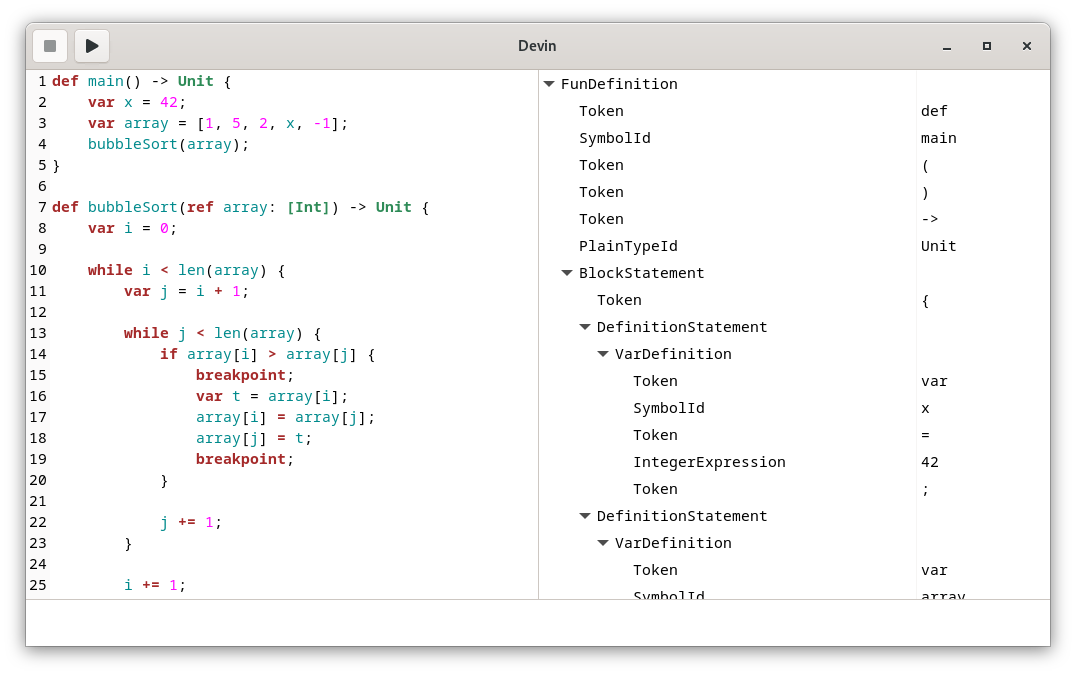
\includegraphics[width=0.9\textwidth]{2.png}
    \caption{The graphical editor associated with Devin}
  \end{figure}

  \section{Language features}

  Devin is an imperative programming language with lexical variable scoping and
  support for recursive function definitions. Syntactically, it's similar to any
  C descendant; among others, it supports variable definition and assignment,
  while loops, do-while loops and branching.

  \subsection{Data types}

  Devin features the following data types:

  \begin{itemize}
    \item \lstinline@Bool@, for the boolean values \lstinline@true@,
    \lstinline@false@;

    \item \lstinline@Int@, for 64-bit integers denoted by sequences of digits
    like \lstinline@42@;

    \item \lstinline@Float@, for double-precision floating-point numbers like
    \lstinline@0.0@ and \lstinline@3.14@. The presence of the fractional part
    distinguishes integers from floats. Contrary to C, exponential notation like
    \lstinline@1E100@ is disallowed;

    \item \lstinline[mathescape]@[$T$]@, for arrays like
    \lstinline@[1, 1, 2, 3, 5, 8, 13, 21, 34, 55]@.
  \end{itemize}

  In addition to the items above, Devin has a \emph{unit type} named
  \lstinline@Unit@; it is inhabited by one value only: \lstinline@unit@. When a
  procedure has side-effects only, it marked as returning \lstinline@Unit@.

  With unit types, there's no need to distinguish between functions which return
  a value and procedures which do not: all which can be called always returns a
  value. One of the advantages of unit types is the uniform treatment
  assignments to calls. While unit types are traditionally used in functional
  programming languages, some recent imperative languages like Kotlin and Rust
  incorporate this feature as well.

  \subsection{Built-in operators}

  Booleans support the usual operations of negation, conjunction, disjunction
  and exclusive disjunction.

  Like many languages, boolean binary operators are evaluated lazily: the right
  operand is only evaluated if the left operand doesn't already determine the
  truthfulness of the whole expression.

  \begin{table}[h]
    \centering

    \begin{tabular}{|c|c|c|c|}
      \hline

      Description &
      Syntax &
      C equivalent &
      Semantic meaning \\
      \hline

      Negation &
      \lstinline[mathescape]@not $p$@ &
      \lstinline[mathescape]@!$p$@ &
      $\lnot p$ \\

      Conjunction &
      \lstinline[mathescape]@$p$ and $q$@ &
      \lstinline[mathescape]@$p$ && $q$@ &
      $p \land q$ \\

      Disjunction &
      \lstinline[mathescape]@$p$ or $q$@ &
      \lstinline[mathescape]@$p$ || $q$@ &
      $p \lor q$ \\

      Exclusive disjunction &
      \lstinline[mathescape]@$p$ xor $q$@ &
      \lstinline[mathescape]@$p$ != $q$@ &
      $\left(p \land \lnot q\right) \lor \left(\lnot p \land q\right)$ \\
      \hline
    \end{tabular}

    \caption{Boolean operators}
  \end{table}

  Integers and floating-point numbers support addition, subtraction,
  multiplication and division. For integers (but not floats), there's the modulo
  operation.

  Binary arithmetic operations require both operands to be of the same type:
  there are no implicit type conversions.

  Division (operator \lstinline@/@) behaves differently depending on the types
  of the operands. In any case, the result of arithmetic operations has the same
  type as their operands.

  \begin{table}[h]
    \centering

    \begin{tabular}{|c|c|c|}
      \hline

      Description &
      Syntax &
      Semantic meaning \\
      \hline

      Negation &
      \lstinline[mathescape]@-$x$@ &
      $-x$ \\

      Identity &
      \lstinline[mathescape]@+$x$@ &
      $+x$ \\

      Addition &
      \lstinline[mathescape]@$x$ + $y$@ &
      $x + y$ \\

      Subtraction &
      \lstinline[mathescape]@$x$ - $y$@ &
      $x - y$ \\

      Multiplication &
      \lstinline[mathescape]@$x$ * $y$@ &
      $x \times y$ \\

      Integer division &
      \lstinline[mathescape]@$n$ / $m$@ &
      $\lfloor n \div m \rfloor$ \\

      Floating-point division &
      \lstinline[mathescape]@$x$ / $y$@ &
      $x \div y$ \\

      Modulo &
      $n$\lstinline@ % @$m$ &
      $n - m \times \lfloor n \div m \rfloor$ \\
      \hline
    \end{tabular}

    \caption{Arithmetic operators}
  \end{table}

  Pairs of numbers can be compared with the expressions
  \lstinline[mathescape]@$x$ < $y$@, \lstinline[mathescape]@$x$ <= $y$@,
  \lstinline[mathescape]@$x$ > $y$@, \lstinline[mathescape]@$x$ >= $y$@.
  Equality between any two values can be tested with
  \lstinline[mathescape]@$x$ == $y$@ and \lstinline[mathescape]@$x$ != $y$@.

  \begin{table}[h]
    \centering

    \begin{tabular}{|c|c|c|}
      \hline

      Description &
      Syntax &
      Semantic meaning \\
      \hline

      \multirow{4}{*}{Comparison} &
      \lstinline[mathescape]@$x$ > $y$@ &
      $x < y$ \\

      &
      \lstinline[mathescape]@$x$ <= $y$@ &
      $x \leq y$ \\

      &
      \lstinline[mathescape]@$x$ > $y$@ &
      $x > y$ \\

      &
      \lstinline[mathescape]@$x$ >= $y$@ &
      $x \geq y$ \\

      \multirow{2}{*}{Equality} &
      \lstinline[mathescape]@$x$ == $y$@ &
      $x \equiv y$ \\

      &
      \lstinline[mathescape]@$x$ != $y$@ &
      $x \not\equiv y$ \\
      \hline
    \end{tabular}

    \caption{Equality and comparison operators}
  \end{table}

  Variables and array elements can be assigned to with the \lstinline@=@
  operator. Like many languages, Devin features a few shorthands as well.

  \begin{table}[h]
    \centering

    \begin{tabular}{|c|c|c|}
      \hline

      Description &
      Syntax &
      Semantic meaning \\
      \hline

      Plain assignment &
      \lstinline[mathescape]@$x$ = $y$@ &
      $x \leftarrow y$ \\

      \multirow{5}{*}{Assignment shorthand} &
      \lstinline[mathescape]@$x$ += $y$@ &
      \lstinline[mathescape]@$x$ = $x$ + $y$@ \\

      &
      \lstinline[mathescape]@$x$ -= $y$@ &
      \lstinline[mathescape]@$x$ = $x$ - $y$@ \\

      &
      \lstinline[mathescape]@$x$ *= $y$@ &
      \lstinline[mathescape]@$x$ = $x$ * $y$@ \\

      &
      \lstinline[mathescape]@$x$ /= $y$@ &
      \lstinline[mathescape]@$x$ = $x$ / $y$@ \\

      &
      \lstinline[mathescape]@$x$ %= $y$@ &
      \lstinline[mathescape]@$x$ = $x$ % $y$@ \\
      \hline
    \end{tabular}

    \caption{Assignment operators}
    \label{table:assignmentoperators}
  \end{table}

  \section{Working with arrays}

  Arrays support the following operations:

  \begin{itemize}
    \item \emph{Element access}: \lstinline[mathescape]@$a$[$n$]@, where $a$
    denotes an array and $n$ an integer index. The expression retrieves the
    $n$-th element of the array. Like in most programming languages, the first
    element of the array has index $0$.

    \item \emph{Length information}: \lstinline[mathescape]@len $a$@. The
    expression returns the number of elements contained in the array $a$.

    \item \emph{Concatenation}: \lstinline[mathescape]@$a$ + $b$@. The
    expression yields a new array containing the elements of $a$ concatenated
    with the elements of $b$;

    \item \emph{Repetition}: \lstinline[mathescape]@$a$ * $n$@ or
    \lstinline[mathescape]@$n$ * $a$@. Equivalent to concatenating $a$ to itself
    $n$ times. \\
    Zero-initialized arrays of size $n$ can be generated with the expression
    \lstinline[mathescape]@[0] * $n$@.
  \end{itemize}

  \subsection{Variable definitions and scoping}

  Variables can be defined using statements of the form
  \lstinline[mathescape]@var $x$ = $y$@, where $x$ is an identifier and $y$ is
  an expression. The type of of the new variable $x$ is inferred from $y$.
  Variables can be defined at any point, whether globally or as function locals.
  Their visibility extends from the point of their definition onward.

  Devin is \emph{block-structured}: it allows for the creation of blocks,
  including blocks nested within other blocks. Variables are lexically scoped:
  they can't be accessed from outside the block they are defined in. As in C, a
  block consists of a sequence of statements wrapped between a pair of curly
  braces (\lstinline@{@, \lstinline@}@). Statements are always terminated with
  semicolons.

  \begin{lstlisting}[
    float=h,
    gobble=4,
    basicstyle=\ttfamily\small,
    caption={Devin's scoping rules visualized}
  ]
    def rotateRight(ref array) -> Unit {
        if len array > 0 {
            var i = len array - 1;
            var t = array[i];

            while i > 0 {
                array[i] = array[i - 1];
                i -= 1;
            }

            array[0] = t;
        }  // 'i', 't' go out of scope
    }  // 'array' goes out of scope
  \end{lstlisting}

  \subsection{Branching and looping mechanisms}

  The following two looping constructs are supported:

  \begin{itemize}
    \item \emph{While loops} in the form \lstinline[mathescape]@while $p$ $s$@.
    This construct runs the statement $s$ as long as the expression $p$ is true;

    \item \emph{Do-while loops} in the form
    \lstinline[mathescape]@do $s$ while $p$@. This construct runs $s$ once;
    then, it re-runs $s$ as long as $p$ is true.
  \end{itemize}

  Conditional code execution is supported through statements of the form
  \lstinline[mathescape]@if $p$ $s_1$@ and
  \lstinline[mathescape]@if $p$ $s_1$ else $s_2$@, where $p$ is a boolean
  predicate and $s_1$ and $s_2$ are statements.

  \subsection{Assertions}

  Devin provides a mechanism for asserting that predicates evaluate to
  \lstinline@true@ at runtime; if they are not, an error is generated, causing
  program termination. Assertions can be used to check internal assumptions or
  to guard against violation of function contracts, among other things.

  For example, the assertion \lstinline@assert n >= 0@ can be used as the first
  statement of a function calculating the factorial of \lstinline@n@, as the
  result not defined if $\text{\lstinline@n@} < 0$.

  \subsection{Procedure definition and application}

  Procedures can be defined either globally or within other procedures. They
  obey to the same scoping rules as variables. The entry point for Devin
  programs is a global procedure named \lstinline@main@; it must take no
  arguments.

  The syntax for calling procedures is the same as in C:
  \lstinline[mathescape]@$f$()@ calls $f$ with zero arguments,
  \lstinline[mathescape]@$g$($x$)@ calls $g$ with a single argument,
  \lstinline[mathescape]@$h$($x$, $y$)@ calls $h$ with two arguments, and so on.

  The evaluation strategy of Devin is eager; arguments are evaluated from left
  to right. By default, procedure arguments are passed by value; with the
  \lstinline@ref@ keyword, they can be passed by reference instead.

  \subsection{Optional types}

  A peculiar feature of Devin is that of \emph{optional types}. With optional
  types, the semantic of the language doesn't depend on the static type
  system~\cite{bracha_2004}. A notable example of an optionally typed language
  is Python. With this feature, type annotations can be omitted from Devin
  programs. Type checking is not performed on terms where type annotations are
  missing. If no type annotations are provided, Devin becomes dynamically typed.

  \begin{lstlisting}[
    float=h,
    gobble=4,
    basicstyle=\ttfamily\small,
    caption={Optional types exemplified}
  ]
    def swap1(ref array: [Int], i: Int, j: Int) -> Unit {
        var t = array[i];
        array[i] = array[j];
        array[j] = t;
    }

    // Note: 'swap2' is more general than 'swap1', as it can be used with any array
    def swap2(ref array, i, j) {
        var t = array[i];
        array[i] = array[j];
        array[j] = t;
    }
  \end{lstlisting}

  \section{Editor features}
  \label{section:editorfeatures}

  Devin is bundled with a code editing UI built upon GTK+, a popular library for
  creating graphical user interfaces. GTK+ works on Windows, macOS and many
  UNIX-like platforms~\cite{gtk+}. Code editing is supported by GtkSourceView, a
  library that extends the GTK+ framework for text editing and support for
  configurable syntax highlighting.

  Other than syntax highlighting, Devin's editor features error reporting: both
  syntactic and semantic errors are displayed according to their position within
  the source code.

  \begin{figure}[h]
    \centering
    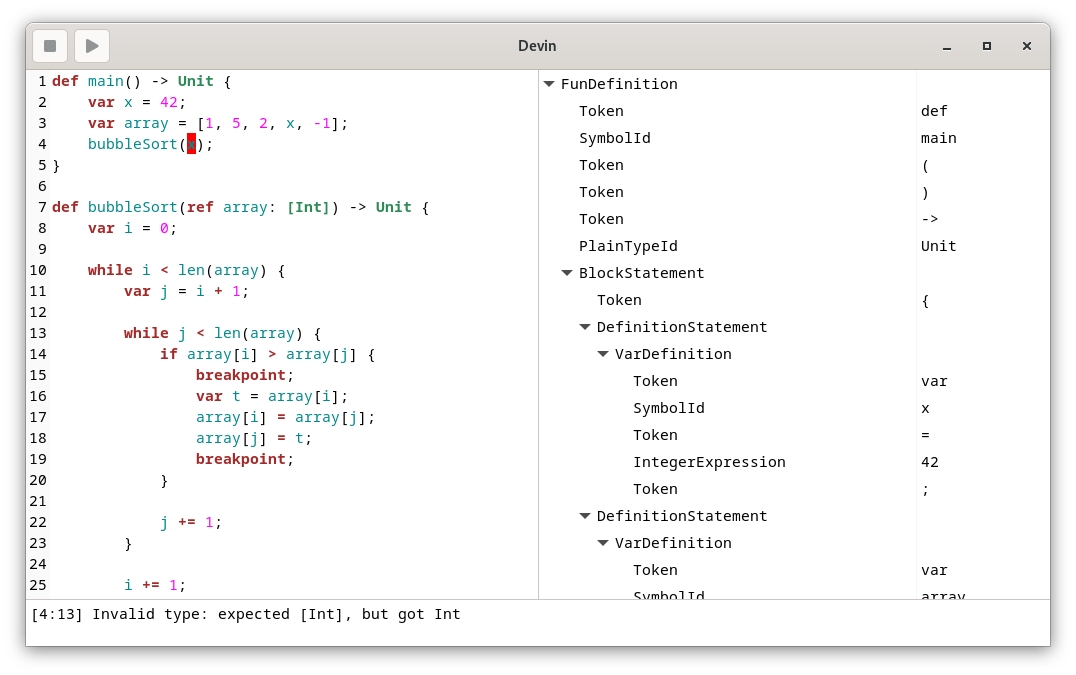
\includegraphics[width=\textwidth]{4.png}
    \caption{Semantic error reporting and highlighting}
  \end{figure}

  Once a valid program has been written, it can be run by clicking the
  $\blacktriangleright$ button. The state of execution can be observed with
  debug statements; these signal the evaluator to pause execution and display
  the current \emph{runtime stack}---the data structure which maps variables and
  function arguments to their values. Each time a function gets called, a new
  \emph{frame} is pushed onto the stack; it contains associations between the
  parameter names and the passed values. Variable definitions within the called
  function add new associations to the newly pushed frame. When the called
  function returns, the topmost frame is popped off the stack and execution
  continues normally.

  Devin has been designed with simplicity of implementation in mind. In
  particular, Devin's call stack exhibits two properties:

  \begin{itemize}
    \item Each block pushes a new frame onto the stack: this allows treating
    nested scopes with the same mechanism as function calls. The debugger skips
    visualization of empty frames, as they occur somewhat frequently.

    \item Execution always starts with a non-empty stack containing a single
    frame. This frame binds the names \lstinline@true@ to the truth value,
    \lstinline@false@ to \lstinline@not true@, \lstinline@unit@ to the unit
    value. In practice, this means that \lstinline@true@, \lstinline@false@ and
    \lstinline@unit@ are not special keywords or constants; instead, they are
    ordinary variables. This is a deliberate design decision.
  \end{itemize}

  \begin{figure}[h]
    \centering
    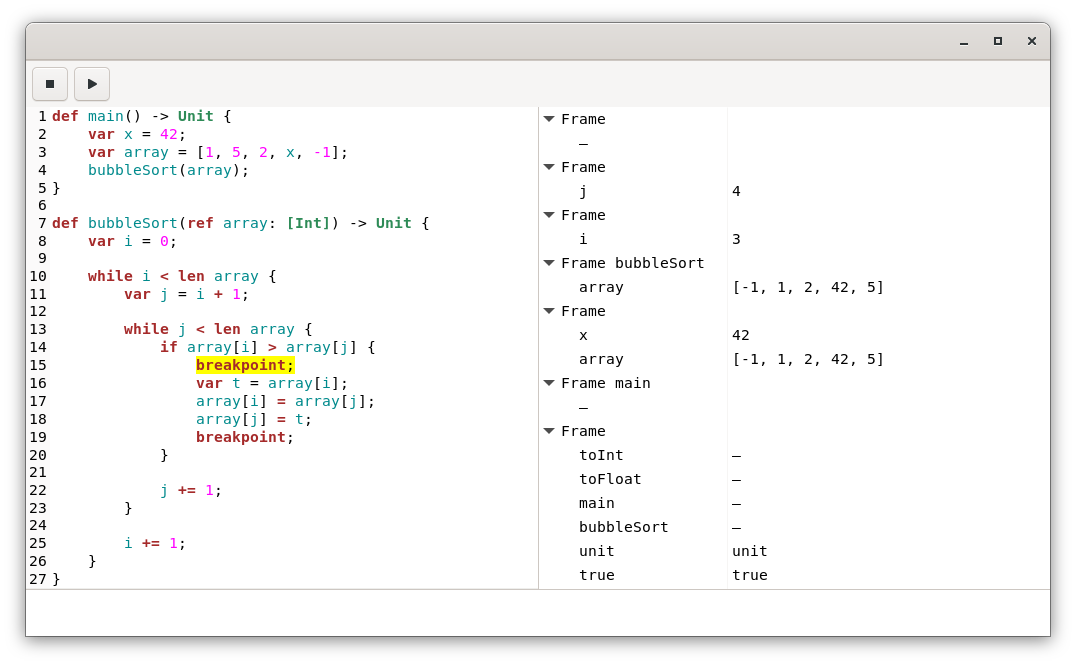
\includegraphics[width=\textwidth]{5.png}
    \caption{The debugger displaying the current state of the stack}
  \end{figure}

  Runtime errors are handled as well. When an error occurs, the offending code
  fragment is highlighted and a message dialog describing the problem is shown
  to the user. Runtime errors include, but are not limited to, index out of
  bounds errors, division by zero, assertion violations.

  \begin{figure}[h]
    \centering
    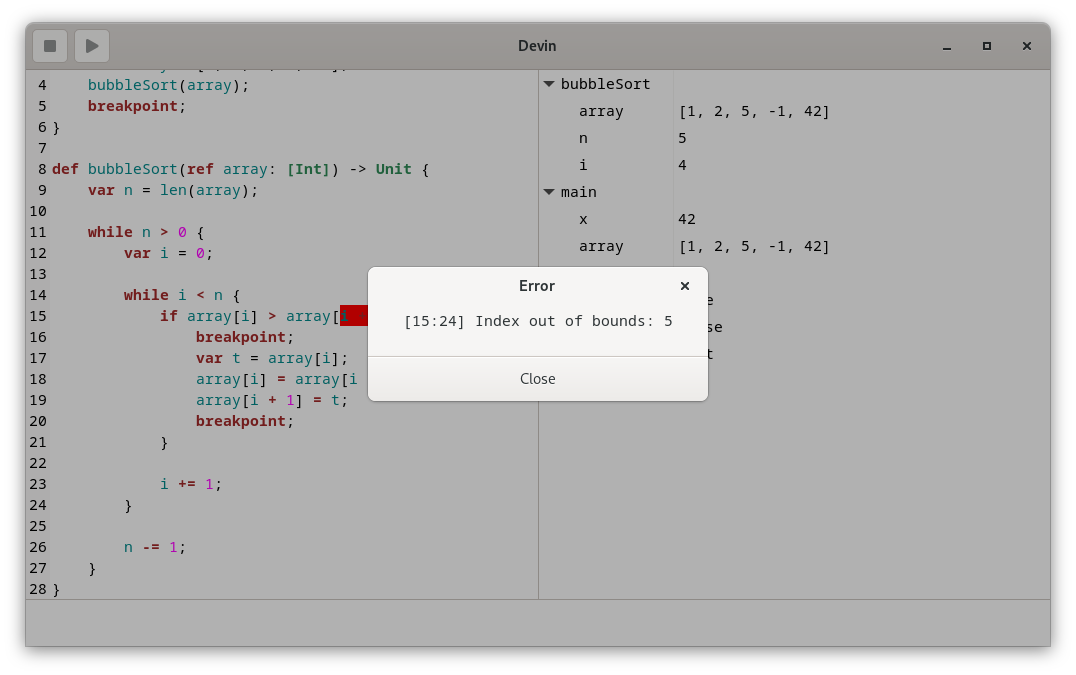
\includegraphics[width=\textwidth]{6.png}
    \caption{Runtime error reporting and highlighting}
  \end{figure}

  \section{Devin's design choices}

  \subsection{Operations between numeric types}

  Addition, subtraction, multiplication, division and modulo are supported only
  if both operands are of the same type. For instance, it isn't legal to sum a
  floating-point number to an integer. While this restriction might seem
  unconventional at first, there is a very specific reason for it.

  In Devin, both integers and floating-point numbers occupy 64 bits. Summing two
  numbers of the same type $T$ yields yet another number of type $T$: nothing
  surprising here. But what should be the result of summing an integer to a
  floating-point number, or vice versa? Many languages take the approach of
  silently converting the integer operand to a floating-point value, and then
  performing the actual summation. Double-precision floating-point format
  numbers as specified in IEEE 754 can't safely represent integers less than
  $-\left(2^{53} - 1\right)$ or greater than $2^{53} - 1$ without loss of
  precision~\cite{mdn}; as such, I argue that a programming language should make
  conversions between integers and floats explicit.

  This design decision is largely inspired by how Haskell deals with numbers.
  Examples of other languages which lack implicit conversions are Go and Rust.

  \subsection{Optional types}

  As discussed previously, type annotations may be omitted at will. As Devin's
  type checker and evaluator are independent, optional types \emph{emerged} as a
  possible additional feature.

  Much can be said regarding the benefits and drawbacks of optional types; a
  completely separate dissertation on its own would be needed to discuss this
  subject alone. There are programming languages with optional types; as
  mentioned, Python is just one example.

  Devin was born due to my own curiosity regarding programming languages and
  their implementation; recreating the next Pascal or C clone is not an
  objective. As optional types are not a common feature and languages shape the
  way we think about solving problems, I decided to add this feature to be
  played around with.

  \chapter{Implementing Devin}

  Devin's implementation spans approximately 4500 lines of code. Knowledge about
  programming in Haskell is required to understand this chapter.

  Devin is entirely written in Haskell. Given the size of its implementation,
  some details are omitted for brevity. In particular, import declarations and
  \lstinline@LANGUAGE@ pragmas are left out for simplicity. Devin's full
  implementation can be found in the appendix.

  In terms of implementation complexity, both the type checker and the evaluator
  are somewhat simpler than the parser. The parser makes much greater use of
  higher order functions and uses multi-parameter type classes, causing some
  syntactical noise on function signatures. Experienced Haskellers should have
  no problems reading the parser's implementation; in any case, I'll describe
  parsing last.

  \section{The syntax tree}

  As mentioned, Devin's syntax tree stores enough information to perform syntax
  highlighting. Given a node in the tree, it is always possible to determine its
  position within the parsed source code. Only leaf nodes store their positions
  directly; the positions of non-leaf nodes can be computed by considering their
  first and last children.

  Two leaf nodes commonly used across Devin's syntax tree are
  \lstinline@SymbolId@ and \lstinline@Token@. They store information about
  identifiers (e.g.\ \lstinline@x@, \lstinline@Int@) and tokens (e.g.\
  \lstinline@{@, \lstinline@}@, \lstinline@->@) respectively. They are defined
  as follows:

  \begin{lstlisting}[gobble=4,basicstyle=\ttfamily\small]
    data SymbolId = SymbolId {name :: String, interval :: (Int, Int)}

    data Token = Token {interval :: (Int, Int)}
  \end{lstlisting}

  \subsection{Representing expressions}

  Devin supports 4 unary operators: \lstinline@+@, \lstinline@-@,
  \lstinline@not@, \lstinline@len@. Unary operators are represented by the
  algebraic data type \lstinline@UnaryOperator@, which is defined as follows:\

  \begin{lstlisting}[gobble=4,basicstyle=\ttfamily\small]
    data UnaryOperator
      = PlusOperator {interval :: (Int, Int)}
      | MinusOperator {interval :: (Int, Int)}
      | NotOperator {interval :: (Int, Int)}
      | LenOperator {interval :: (Int, Int)}
  \end{lstlisting}

  The 20 binary operators \lstinline@+@, \lstinline@-@, \lstinline@*@,
  \lstinline@/@, \lstinline@%@, \lstinline@==@,
  \lstinline@!=@, \lstinline@<@, \lstinline@<=@, \lstinline@>@, \lstinline@>=@,
  \lstinline@and@, \lstinline@or@, \lstinline@xor@, \lstinline@=@,
  \lstinline@+=@, \lstinline@-=@, \lstinline@*=@, \lstinline@/=@,
  \lstinline@%=@ are represented by the
  type \lstinline@BinaryOperator@:

  \begin{lstlisting}[gobble=4,basicstyle=\ttfamily\small]
    data BinaryOperator
      = AddOperator {interval :: (Int, Int)}
      | SubtractOperator {interval :: (Int, Int)}
      | MultiplyOperator {interval :: (Int, Int)}
      | DivideOperator {interval :: (Int, Int)}
      | ModuloOperator {interval :: (Int, Int)}
      | EqualOperator {interval :: (Int, Int)}
      | NotEqualOperator {interval :: (Int, Int)}
      | LessOperator {interval :: (Int, Int)}
      | LessOrEqualOperator {interval :: (Int, Int)}
      | GreaterOperator {interval :: (Int, Int)}
      | GreaterOrEqualOperator {interval :: (Int, Int)}
      | AndOperator {interval :: (Int, Int)}
      | OrOperator {interval :: (Int, Int)}
      | XorOperator {interval :: (Int, Int)}
      | PlainAssignOperator {interval :: (Int, Int)}
      | AddAssignOperator {interval :: (Int, Int)}
      | SubtractAssignOperator {interval :: (Int, Int)}
      | MultiplyAssignOperator {interval :: (Int, Int)}
      | DivideAssignOperator {interval :: (Int, Int)}
      | ModuloAssignOperator {interval :: (Int, Int)}
  \end{lstlisting}

  Literals, numbers and variables are the simplest kinds of expressions, as they
  are atomic. More complex expressions can be built from simpler ones: for
  example, a binary expression is constructed by two sub-expressions and a
  binary operator.

  Expressions are described by a single algebraic data type:
  \lstinline@Expression@. Opening and closing parentheses are stored in the
  syntax tree. As a convention, parentheses are always identified by the
  \lstinline@open@ and \lstinline@close@ fields, regardless of the kind:
  round, square or curly.

  \begin{lstlisting}[gobble=4,basicstyle=\ttfamily\small]
    data Expression where
      VarExpression :: {
        varName :: String,
        interval :: (Int, Int)
      } -> Expression

      IntegerExpression :: {
        integer :: Integer,
        interval :: (Int, Int)
      } -> Expression

      RationalExpression :: {
        rational :: Rational,
        interval :: (Int, Int)
      } -> Expression

      ArrayExpression :: {
        open :: Token,
        elems :: [Expression],
        commas :: [Token],
        close :: Token
      } -> Expression

      AccessExpression :: {
        array :: Expression,
        open :: Token,
        index :: Expression,
        close :: Token
      } -> Expression

      CallExpression :: {
        funId :: SymbolId,
        open :: Token,
        args :: [Expression],
        commas :: [Token],
        close :: Token
      } -> Expression

      UnaryExpression :: {
        unary :: UnaryOperator,
        operand :: Expression
      } -> Expression

      BinaryExpression :: {
        left :: Expression,
        binary :: BinaryOperator,
        right :: Expression
      } -> Expression

      ParenthesizedExpression :: {
        open :: Token,
        inner :: Expression,
        close :: Token
      } -> Expression
  \end{lstlisting}

  \subsection{Representing statements}

  Any expression followed by a semicolon becomes a statement. The type
  \lstinline@Statement@ represents these, along with if, while, do-while,
  return, assert, debug and block statements.

  In any point in which a statement may occur, a variable or function definition
  can be placed instead. The data constructor \lstinline@DefinitionStatement@
  represents this idea.

  \begin{lstlisting}[gobble=4,basicstyle=\ttfamily\small]
    data Statement where
      DefinitionStatement :: {
        definition :: Definition
      } -> Statement

      ExpressionStatement :: {
        value :: Expression,
        semicolon :: Token
      } -> Statement

      IfStatement :: {
        ifKeyword :: Token,
        predicate :: Expression,
        trueBranch :: Statement
      } -> Statement

      IfElseStatement :: {
        ifKeyword :: Token,
        predicate :: Expression,
        trueBranch :: Statement,
        elseKeyword :: Token,
        falseBranch :: Statement
      } -> Statement

      WhileStatement :: {
        whileKeyword :: Token,
        predicate :: Expression,
        body :: Statement
      } -> Statement

      DoWhileStatement :: {
        doKeyword :: Token,
        body :: Statement,
        whileKeyword :: Token,
        predicate :: Expression,
        semicolon :: Token
      } -> Statement

      ReturnStatement :: {
        returnKeyword :: Token,
        result :: Maybe Expression,
        semicolon :: Token
      } -> statement

      AssertStatement :: {
        assertKeyword :: Token,
        predicate :: Expression,
        semicolon :: Token
      } -> Statement

      DebugStatement :: {
        debugKeyword :: Token,
        semicolon :: Token
      } -> Statement

      BlockStatement :: {
        open :: Token,
        statements :: [Statement],
        close :: Token
      } -> Statement
  \end{lstlisting}

  \subsection{Representing variable and function definitions}

  Devin's function definitions may include signatures with explicit types. The
  syntax for array types is that of a type wrapped in square brackets, as in
  \lstinline@[Int]@ or \lstinline@[[Float]]@. The arbitrary syntactical nesting
  of paired square brackets around a type is permitted by the algebraic data
  type \lstinline@TypeId@:

  \begin{lstlisting}[gobble=4,basicstyle=\ttfamily\small]
    data TypeId
      = PlainTypeId {name :: String, interval :: (Int, Int)}
      | ArrayTypeId {open :: Token, innerTypeId :: TypeId, close :: Token}
  \end{lstlisting}

  Variables and functions definitions are given by \lstinline@VarDefinition@ and
  \lstinline@FunDefinition@.

  \begin{lstlisting}[gobble=4,basicstyle=\ttfamily\small]
    data Definition where
      VarDefinition :: {
        varKeyword :: Token,
        varId :: SymbolId,
        equalSign :: Token,
        value :: Expression,
        semicolon :: Token
      } -> Definition

      FunDefinition :: {
        defKeyword :: Token,
        funId :: SymbolId,
        open :: Token,
        params :: [(Maybe Token, SymbolId, Maybe (Token, TypeId))],
        commas :: [Token],
        close :: Token,
        returnInfo :: Maybe (Token, TypeId),
        body :: Statement
      } -> Definition
  \end{lstlisting}

  \section{Representing semantic errors}

  Both the evaluator and the type checker require some data type to represent
  errors. Runtime errors, like division by zero, are raised by the evaluator.
  Static analysis errors, like a missing return statement, are reported by the
  type checker. As some errors are common to both phases, a single algebraic
  data type is used:

  \begin{lstlisting}[gobble=4,basicstyle=\ttfamily\small]
    data Error where
      UnknownVar :: {
        varName :: String,
        interval :: (Int, Int)
      } -> Error

      UnknownFun :: {
        funName :: String,
        interval :: (Int, Int)
      } -> Error

      UnknownType :: {
        typeName :: String,
        interval :: (Int, Int)
      } -> Error

      InvalidUnary :: {
        unary :: UnaryOperator,
        operandT :: Type
      } -> Error

      InvalidBinary :: {
        binary :: BinaryOperator,
        leftT :: Type,
        rightT :: Type
      } -> Error

      InvalidType :: {
        expression :: Expression,
        expectedT :: Type,
        actualT :: Type
      } -> Error

      -- Static errors:

      MissingReturnValue :: {
        statement :: Statement,
        expectedT :: Type
      } -> Error

      MissingReturnStatement :: {
        funId :: SymbolId
      } -> Error

      -- Runtime errors:

      IntegerOverflow :: {
        expression :: Expression
      } -> Error

      DivisionByZero :: {
        expression :: Expression
      } -> Error

      IndexOutOfBounds :: {
        expression :: Expression,
        value :: Int64
      } -> Error

      InvalidArgCount :: {
        expression :: Expression,
        expected :: Int,
        actual :: Int
      } -> Error

      AssertionFailed :: {
        statement :: Statement
      } -> Error
  \end{lstlisting}

  \section{The type checker}

  At high level, type checking is performed by a set of functions that operate
  on an \emph{environment}, a data structure which associates identifiers to
  types. The environment is used to assert that function calls and variable
  usages are valid within their context.

  The module \lstinline@Devin.Type@ provides the structures necessary to
  represent types. The data constructors \lstinline@Unit@, \lstinline@Bool@,
  \lstinline@Int@, \lstinline@Float@ and \lstinline@Array@ correspond to Devin's
  supported types. To aid the type checker, two other data constructors are
  provided, both of which indicate some sort of error: \lstinline@Unknown@ and
  \lstinline@Placeholder@. While \lstinline@Unknown@ stands for an unknown type,
  \lstinline@Placeholder@ represents a specific unresolved type. Differentiating
  between between \lstinline@Placeholder@ and \lstinline@Unknown@ allows for
  fine-grained error messages and diagnostics.

  \begin{lstlisting}[gobble=4,basicstyle=\ttfamily\small]
    data Type
      = Unknown
      | Unit
      | Bool
      | Int
      | Float
      | Array Type
      | Placeholder String
  \end{lstlisting}

  To compare types, the relation operator \lstinline@(<:)@ is provided:

  \begin{lstlisting}[gobble=4,basicstyle=\ttfamily\small]
    (<:) :: Type -> Type -> Bool
    t1 <: t2 = isJust (merge t1 t2)

    merge :: Type -> Type -> Maybe Type
    merge Unknown _ = Just Unknown
    merge _ Unknown = Just Unknown
    merge Unit Unit = Just Unit
    merge Bool Bool = Just Bool
    merge Int Int = Just Int
    merge Float Float = Just Float
    merge (Array t1) (Array t2) = Array <$> merge t1 t2
    merge (Placeholder n1) (Placeholder n2) | n1 == n2 = Just (Placeholder n1)
    merge _ _ = Nothing
  \end{lstlisting}

  Given two types, the helper function \lstinline@merge@ yields a type
  compatible to both, if possible. All types except for \lstinline@Unknown@ are
  only compatible with themselves; \lstinline@Unknown@, on the other hand, is
  compatible with all other types.

  The module \lstinline@Devin.Typer@ implements the type checker interface. In
  order to account for Devin's lexical scoping rules, the environment is
  represented as a list of association lists.

  \begin{lstlisting}[gobble=4,basicstyle=\ttfamily\small]
    data Scope = Scope {
      types :: [(String, Type)],
      funs :: [(String, ([Type], Type))],
      vars :: [(String, Type)]
    }

    type Environment = [Scope]

    data Typer a = Typer {runTyper :: Environment -> (a, Environment, [Error])}
      deriving Functor
  \end{lstlisting}

  In the listing above, \lstinline@Typer@ wraps a function which takes an
  \lstinline@Environment@ and returns a new environment and a potentially empty
  list of \lstinline@Error@s, along with a result of some kind.
  \lstinline@deriving Functor@ instructs GHC to automatically generate an
  implementation for the function
  \lstinline@fmap :: (a -> b) -> Typer a -> Typer b@.

  Below, implementations for \lstinline@pure@, \lstinline@liftA2@,
  \lstinline@(>>=)@ are provided. Implementing those functions, along with
  \lstinline@fmap@, makes \lstinline@Typer@ a monad.

  \begin{lstlisting}[gobble=4,basicstyle=\ttfamily\small]
    instance Applicative Typer where
      pure :: a -> Typer a
      pure x = Typer (\env -> (x, env, []))

      liftA2 :: (a -> b -> c) -> Typer a -> Typer b -> Typer c
      liftA2 f mx my = Typer $ \env ->
        let (x, env', errors1) = runTyper mx env
            (y, env'', errors2) = runTyper my env'
         in (f x y, env'', errors1 ++ errors2)

    instance Monad Typer where
      (>>=) :: Typer a -> (a -> Typer b) -> Typer b
      mx >>= f = Typer $ \env ->
        let (x, env', errors1) = runTyper mx env
            (y, env'', errors2) = runTyper (f x) env'
         in (y, env'', errors1 ++ errors2)
  \end{lstlisting}

  Next, some utility functions are defined. The function \lstinline@defineType@
  binds a name to a \lstinline@Type@ (the binding is added to the current
  environment). Its dual, \lstinline@lookupType@, looks up to which type a name
  is bound. \lstinline@lookupType@ searches the current environment first; if no
  bindings are found, the parent environment is scanned next.

  \begin{lstlisting}[gobble=4,basicstyle=\ttfamily\small]
    defineType :: String -> Type -> Typer Type
    defineType name t = Typer $ \case
      [] -> (t, [Scope [(name, t)] [] []], [])

      scope : parents ->
        let types' = (name, t) : types scope
         in (t, scope {types = types'} : parents, [])

    lookupType :: String -> Typer (Maybe (Type, Int))
    lookupType name = Typer (\env -> (go 0 env, env, []))
      where
        go _ [] = Nothing

        go depth (Scope {types} : parents) = case lookup name types of
          Just t -> Just (t, depth)
          Nothing -> go (depth + 1) parents
  \end{lstlisting}

  The functions \lstinline@defineFunSignature@ and
  \lstinline@lookupFunSignature@ define and lookup associations between names
  and function signatures represented by the tuple \lstinline@([Type], Type)@.
  The first element of the tuple is the list of parameter types, the second is
  the return type.

  \begin{lstlisting}[gobble=4,basicstyle=\ttfamily\small]
    defineFunSignature :: String -> ([Type], Type) -> Typer ()
    defineFunSignature name signature = Typer $ \case
      [] -> ((), [Scope [] [(name, signature)] []], [])

      scope : parents ->
        let funs' = (name, signature) : funs scope
         in ((), scope {funs = funs'} : parents, [])

    lookupFunSignature :: String -> Typer (Maybe (([Type], Type), Int))
    lookupFunSignature name = Typer (\env -> (go 0 env, env, []))
      where
        go _ [] = Nothing

        go depth (Scope {funs} : parents) = case lookup name funs of
          Just signature -> Just (signature, depth)
          Nothing -> go (depth + 1) parents
  \end{lstlisting}

  Finally, variables can be defined and looked up with \lstinline@defineVarType@
  and \lstinline@lookupVarType@.

  \begin{lstlisting}[gobble=4,basicstyle=\ttfamily\small]
    defineVarType :: String -> Type -> Typer ()
    defineVarType name t = Typer $ \case
      [] -> ((), [Scope [] [] [(name, t)]], [])

      scope : parents ->
        let vars' = (name, t) : vars scope
         in ((), scope {vars = vars'} : parents, [])

    lookupVarType :: String -> Typer (Maybe (Type, Int))
    lookupVarType name = Typer (\env -> (go 0 env, env, []))
      where
        go _ [] = Nothing

        go depth (Scope {vars} : parents) = case lookup name vars of
          Just t -> Just (t, depth)
          Nothing -> go (depth + 1) parents
  \end{lstlisting}

  Functions to remove previously defined associations could be implemented;
  however, this is not necessary. Instead, the function \lstinline@withNewScope@
  runs another \lstinline@Typer@ on a modified environment where an empty
  \lstinline@Scope@ is added; when the function returns, the previous
  environment is restored.

  \begin{lstlisting}[gobble=4,basicstyle=\ttfamily\small]
    withNewScope :: Typer a -> Typer a
    withNewScope mx = Typer $ \env ->
      let (x, env', errors) = runTyper mx (Scope [] [] [] : env)
       in (x, tail env', errors)
  \end{lstlisting}

  One last function is provided for utility: \lstinline@report@. As its name
  implies, this function reports some \lstinline@Error@; errors are accumulated
  by the \lstinline@Typer@ monad and can be used in successive phases for error
  reporting and highlighting.

  \begin{lstlisting}[gobble=4,basicstyle=\ttfamily\small]
    report :: Error -> Typer ()
    report error = Typer (\env -> ((), env, [error]))
  \end{lstlisting}

  \subsection{Checking expressions}

  Expression related type checking is implemented in the
  \lstinline@Devin.Typers@ module with the
  \lstinline@checkExpression :: Expression -> Typer Type@ function.

  Devin has a rudimentary mechanism for type inference. The type of literal
  expressions is trivially determined by the kind of literal. For variables, a
  lookup in the current environment is performed; if the variable is not bound,
  an error is reported.

  \begin{lstlisting}[gobble=4,basicstyle=\ttfamily\small]
    checkExpression IntegerExpression {} = pure Int

    checkExpression RationalExpression {} = pure Float

    checkExpression VarExpression {varName, interval} =
      lookupVarType varName >>= \case
        Just (t, _) -> pure t

        Nothing -> do
          report (UnknownVar varName interval)
          pure Unknown
  \end{lstlisting}

  For simplicity, the function \lstinline@report'@ is provided for future use.
  It is similar to \lstinline@report@, but its result wraps
  \lstinline@Unknown@ instead of the unit type \lstinline@()@.

  \begin{lstlisting}[gobble=4,basicstyle=\ttfamily\small]
    report' error = do
      report error
      pure Unknown
  \end{lstlisting}

  Inferring the type of arrays requires special care. In general, the type of an
  array is represented by \lstinline[mathescape]@Array $T$@. If all the elements
  of the array have the same type $T_0$, then $T$ can determined to be $T_0$. If
  the array is empty, or if there are at least two elements of the array with
  different types, then $T$ can't be inferred.

  \begin{lstlisting}[gobble=4,basicstyle=\ttfamily\small]
    checkExpression ArrayExpression {elems = []} = pure (Array Unknown)

    checkExpression ArrayExpression {elems = elem : elems} = do
      t <- checkExpression elem
      go elems t

      where
        go [] t = pure (Array t)

        go (elem : elems) t = checkExpression elem >>= \case
          Unknown -> do
            for_ elems checkExpression
            pure (Array Unknown)

          t' | t' <: t -> go elems t

          t' -> do
            report (InvalidType elem t t')
            go elems t
  \end{lstlisting}

  Access to array elements is checked as follows:

  \begin{lstlisting}[gobble=4,basicstyle=\ttfamily\small]
    checkExpression AccessExpression {array, index} = do
      arrayT <- checkExpression array
      indexT <- checkExpression index

      case (arrayT, indexT) of
        (Unknown, Int) -> pure Unknown
        (Unknown, _) -> report' (InvalidType index Int indexT)
        (Array t, Int) -> pure t
        (Array _, _) -> report' (InvalidType index Int indexT)
        (_, _) -> report' (InvalidType array (Array Unknown) arrayT)
  \end{lstlisting}

  Unary arithmetic expressions with the operators \lstinline@+@ and
  \lstinline@-@ are type checked by asserting that the operand is of a numeric
  type. If it is, the result of evaluating the whole expression has the same
  type of the operand.

  \begin{lstlisting}[gobble=4,basicstyle=\ttfamily\small]
    checkExpression UnaryExpression {unary, operand}
      | PlusOperator {} <- unary = do
        operandT <- checkExpression operand

        case operandT of
          Unknown -> pure Unknown
          Int -> pure Int
          Float -> pure Float
          _ -> report' (InvalidUnary unary operandT)

    checkExpression UnaryExpression {unary, operand}
      | MinusOperator {} <- unary = do
        operandT <- checkExpression operand

        case operandT of
          Unknown -> pure Unknown
          Int -> pure Int
          Float -> pure Float
          _ -> report' (InvalidUnary unary operandT)
  \end{lstlisting}

  The boolean \lstinline@not@ is checked in a similar manner:

  \begin{lstlisting}[gobble=4,basicstyle=\ttfamily\small]
    checkExpression UnaryExpression {unary, operand}
      | NotOperator {} <- unary = do
        operandT <- checkExpression operand

        case operandT of
          Unknown -> pure Unknown
          Bool -> pure Bool
          _ -> report' (InvalidUnary unary operandT)
  \end{lstlisting}

  Unary expressions with the operator \lstinline@len@ are valid only if the
  operand is an array. The resulting type is an \lstinline@Int@.

  \begin{lstlisting}[gobble=4,basicstyle=\ttfamily\small]
    checkExpression UnaryExpression {unary, operand}
      | LenOperator {} <- unary = do
        operandT <- checkExpression operand

        case operandT of
          Unknown -> pure Unknown
          Array _ -> pure Int
          _ -> report' (InvalidUnary unary operandT)
  \end{lstlisting}

  As can be seen, there is a certain degree of code repetition within
  \lstinline@checkExpression@. While \emph{DRY} (Don't Repeat Yourself) is
  usually a good software development practice, it does become impractical when
  edge cases have to be considered. For instance, while both binary operators
  \lstinline@+@ and \lstinline@-@ operate on arithmetic types, \lstinline@+@
  also works with arrays. The problem becomes worse in the evaluator, where both
  \lstinline@+@ and \lstinline@and@ compute some result based on their operands,
  but the evaluation strategy of \lstinline@and@ differs from that of
  \lstinline@+@. Source code could certainly be rearranged to avoid some amount
  of repetition; however, it would become less readable to some extent.

  What follows is the implementation to type check expressions with the binary
  operator~\lstinline@/@. Both operands have to be of the same type; if they
  are, the result of evaluating the whole expression has the same type as the
  operands.

  \begin{lstlisting}[gobble=4,basicstyle=\ttfamily\small]
    checkExpression BinaryExpression {left, binary, right}
      | DivideOperator {} <- binary = do
        leftT <- checkExpression left
        rightT <- checkExpression right

        case (leftT, rightT) of
          (Unknown, _) -> pure Unknown
          (_, Unknown) -> pure Unknown
          (Int, Int) -> pure Int
          (Float, Float) -> pure Float
          (_, _) -> report' (InvalidBinary binary leftT rightT)
  \end{lstlisting}

  The binary operators \lstinline@-@ and \lstinline@%@ are type
  checked similarly to \lstinline@/@, except for the fact that
  \lstinline@%@ only accepts operands of type \lstinline@Int@.

  The semantic meaning of the binary operator \lstinline@+@ depends on the type
  of the operands. If both of them are numeric, the operator denotes an
  arithmetic addition; if the operands are arrays, \lstinline@+@ stands for
  array concatenation. Similarly, \lstinline@*@ could indicate both numeric
  multiplication and array repetition. As these operators are overloaded, all
  possibilities have to be considered during type checking.

  \begin{lstlisting}[gobble=4,basicstyle=\ttfamily\small]
    checkExpression BinaryExpression {left, binary, right}
      | AddOperator {} <- binary = do
        leftT <- checkExpression left
        rightT <- checkExpression right

        case (leftT, rightT) of
          (Unknown, _) -> pure Unknown
          (_, Unknown) -> pure Unknown
          (Int, Int) -> pure Int
          (Float, Float) -> pure Float
          (Array t1, Array t2) | Just t <- merge t1 t2 -> pure (Array t)
          (_, _) -> report' (InvalidBinary binary leftT rightT)

    checkExpression BinaryExpression {left, binary, right}
      | MultiplyOperator {} <- binary = do
        leftT <- checkExpression left
        rightT <- checkExpression right

        case (leftT, rightT) of
          (Unknown, _) -> pure Unknown
          (_, Unknown) -> pure Unknown
          (Int, Int) -> pure Int
          (Float, Float) -> pure Float
          (Array t, Int) -> pure (Array t)
          (Int, Array t) -> pure (Array t)
          (_, _) -> report' (InvalidBinary binary leftT rightT)
  \end{lstlisting}

  Values can be compared with the binary operators \lstinline@<@,
  \lstinline@<=@, \lstinline@>@ and \lstinline@>=@. Type checking ensures that
  both operands are of the same numeric type; if they are, expressions with such
  operators yield a \lstinline@Bool@. Type checking is implemented in the
  exactly same way for all four comparison operators:

  \begin{lstlisting}[gobble=4,basicstyle=\ttfamily\small]
    checkExpression BinaryExpression {left, binary, right}
      | LessOperator {} <- binary = do
        leftT <- checkExpression left
        rightT <- checkExpression right

        case (leftT, rightT) of
          (Unknown, _) -> pure Unknown
          (_, Unknown) -> pure Unknown
          (Int, Int) -> pure Bool
          (Float, Float) -> pure Bool
          (_, _) -> report' (InvalidBinary binary leftT rightT)
  \end{lstlisting}

  Equality can be tested between values of any two types. Values of different
  types are deemed to be always different.

  Notice that \lstinline@left@ and \lstinline@right@ are recursively type
  checked even though the result type (\lstinline@Bool@) is known. This is
  important, as failing to check sub-expressions could lead to runtime errors
  during evaluation.

  \begin{lstlisting}[gobble=4,basicstyle=\ttfamily\small]
    checkExpression BinaryExpression {left, binary, right}
      | EqualOperator {} <- binary = do
        checkExpression left
        checkExpression right
        pure Bool

    checkExpression BinaryExpression {left, binary, right}
      | NotEqualOperator {} <- binary = do
        checkExpression left
        checkExpression right
        pure Bool
  \end{lstlisting}

  The operators \lstinline@and@, \lstinline@or@ and \lstinline@xor@ are all
  checked in the same manner.

  \begin{lstlisting}[gobble=4,basicstyle=\ttfamily\small]
    checkExpression BinaryExpression {left, binary, right}
      | AndOperator {} <- binary = do
        leftT <- checkExpression left
        rightT <- checkExpression right

        case (leftT, rightT) of
          (Unknown, _) -> pure Unknown
          (_, Unknown) -> pure Unknown
          (Bool, Bool) -> pure Bool
          (_, _) -> report' (InvalidBinary binary leftT rightT)
  \end{lstlisting}

  Assignments with \lstinline@=@ are checked by verifying that both the left and
  right operands are of the same type. Interestingly, it is not checked whether
  the left-hand side is a variable. As an example, an expression like
  \lstinline@1 = 2@ is considered valid as it would not fail at runtime. The
  reason for a particular behavior is the implementation of the evaluator, which
  for simplicity considers everything to be assignable. The type checker
  could've been programmed to reject such behavior even if it is well defined at
  runtime; however, it could be argued that it is the job of a linter to check
  for such expressions.

  \begin{lstlisting}[gobble=4,basicstyle=\ttfamily\small]
    checkExpression BinaryExpression {left, binary, right}
      | PlainAssignOperator {} <- binary = do
        leftT <- checkExpression left
        rightT <- checkExpression right

        if leftT <: rightT then
          pure leftT
        else
          report' (InvalidBinary binary leftT rightT)
  \end{lstlisting}

  Expressions with the binary operators \lstinline@+=@, \lstinline@-=@,
  \lstinline@*=@, \lstinline@/=@,
  \lstinline@%=@ are type checked considering the shorthands detailed in table
  \ref{table:assignmentoperators}.

  The type resulting from function invocations is determined by looking up the
  callee's signature. If a call refers to an unbound identifier, or if the wrong
  number of arguments is provided, or if an argument has the wrong type, an
  error is reported.

  \begin{lstlisting}[gobble=4,basicstyle=\ttfamily\small]
    checkExpression CallExpression {funId = SymbolId {name, interval}, args} =
      lookupFunSignature name >>= \case
        Just ((paramTs, returnT), _) -> go 0 args paramTs
          where
            go _ [] [] = pure returnT

            go n (arg : args) (paramT : paramTs) = do
              argT <- checkExpression arg
              unless (argT <: paramT) (report (InvalidType arg paramT argT))
              go (n + 1) args paramTs

            go n args paramTs = do
              let expected = n + length paramTs
              let actual = n + length args
              report' (InvalidArgCount expression expected actual)

        Nothing -> report' (UnknownFun name interval)
  \end{lstlisting}

  \subsection{Checking statements}

  The function \lstinline@checkStatement :: Type -> Statement -> Typer Bool@
  performs type \linebreak checking on statements. A type must be provided: on
  return statements, \lstinline@checkStatement@ verifies that the returned value
  is of the given type.

  Inside procedures, return statements may signal control to be returned the
  callee. The function \lstinline@checkStatement@ wraps a \lstinline@Bool@ which
  is \lstinline@True@ if control is guaranteed to be returned to the callee and
  \lstinline@False@ otherwise.

  Expression and definition statements are trivial to check. In both cases, type
  checking is delegated to the relevant function. \lstinline@checkDefinitions@
  is defined in the next section.

  \begin{lstlisting}[gobble=4,basicstyle=\ttfamily\small]
    checkStatement _ ExpressionStatement {value} = do
      checkExpression value
      pure False

    checkStatement _ DefinitionStatement {definition} = do
      checkDefinitions [definition]
      pure False
  \end{lstlisting}

  If-else statements are type checked by asserting that the predicate is a
  boolean and recursively checking both possible execution paths. If both
  branches return control, then the if-else statement surely returns control as
  well.

  \begin{lstlisting}[gobble=4,basicstyle=\ttfamily\small]
    checkStatement expectedT IfElseStatement {predicate, trueBranch, falseBranch} = do
      t <- checkExpression predicate
      unless (t <: Bool) (report (InvalidType predicate Bool t))
      trueBranchDoesReturn <- withNewScope (checkStatement expectedT trueBranch)
      falseBranchDoesReturn <- withNewScope (checkStatement expectedT falseBranch)
      pure (trueBranchDoesReturn && falseBranchDoesReturn)
  \end{lstlisting}

  For if statements without \lstinline@else@ it can't be deduced whether control
  is returned, as the value of the predicate is only known at runtime.

  \begin{lstlisting}[gobble=4,basicstyle=\ttfamily\small]
    checkStatement expectedT IfStatement {predicate, trueBranch} = do
      t <- checkExpression predicate
      unless (t <: Bool) (report (InvalidType predicate Bool t))
      withNewScope (checkStatement expectedT trueBranch)
      pure False
  \end{lstlisting}

  Both while and do-while statements are checked with the considerations similar
  to if and if-else statements respectively.

  \begin{lstlisting}[gobble=4,basicstyle=\ttfamily\small]
    checkStatement expectedT WhileStatement {predicate, body} = do
      t <- checkExpression predicate
      unless (t <: Bool) (report (InvalidType predicate Bool t))
      withNewScope (checkStatement expectedT body)
      pure False

    checkStatement expectedT DoWhileStatement {body, predicate} = do
      doesReturn <- withNewScope (checkStatement expectedT body)
      t <- checkExpression predicate
      unless (t <: Bool) (report (InvalidType predicate Bool t))
      pure doesReturn
  \end{lstlisting}

  Return statements are checked by asserting that the returned value has the
  correct type. If the return value is omitted, it is assumed that
  \lstinline@unit@ is returned instead.

  \begin{lstlisting}[gobble=4,basicstyle=\ttfamily\small]
    checkStatement expectedT ReturnStatement {result = Just result} = do
      t <- checkExpression result
      unless (t <: expectedT) (report (InvalidType result expectedT t))
      pure True

    checkStatement expectedT statement @ ReturnStatement {result = Nothing} = do
      unless (Unit <: expectedT) (report (MissingReturnValue statement expectedT))
      pure True
  \end{lstlisting}

  Assertions are type checked by verifying whether the predicate is of type
  \lstinline@Bool@.

  \begin{lstlisting}[gobble=4,basicstyle=\ttfamily\small]
    checkStatement _ AssertStatement {predicate} = do
      t <- checkExpression predicate
      unless (t <: Bool) (report (InvalidType predicate Bool t))
      pure False
  \end{lstlisting}

  For debug statements, nothing needs to be done.

  \begin{lstlisting}[gobble=4,basicstyle=\ttfamily\small]
    checkStatement _ DebugStatement {} = pure False
  \end{lstlisting}

  Finally, blocks are type checked by recursively checking all statements they
  contain. It is deduced that a block returns control if at least one of it
  statements does.

  Devin's syntactical scoping rules have to be considered: declarations in a
  block have to be discarded at the end of its scope. Thus, statements and
  declarations within blocks have to be type checked in a new temporary
  environment, using the \lstinline@withNewScope@ function.

  \begin{lstlisting}[gobble=4,basicstyle=\ttfamily\small]
    checkStatement expectedT BlockStatement {statements} = withNewScope $ do
      for_ statements $ \case
        DefinitionStatement {definition} -> checkDefinition1 definition
        _ -> pure ()

      foldlM f False statements

      where
        f doesReturn statement = (doesReturn ||) <$> check statement

        check DefinitionStatement {definition} = do
          checkDefinition2 definition
          pure False

        check statement = checkStatement expectedT statement
  \end{lstlisting}

  \subsection{Checking variable and function definitions}

  Given a block, definitions are checked using a two-pass strategy. The first
  pass looks for function definitions and stores the relevant signatures in the
  environment; the body of the functions is not checked at this stage. The
  second pass processes variable definitions and statements within those
  function definitions. Without two-pass type checking, mutually recursive
  function definitions would not be supported---at least not without a mechanism
  like C's forward declarations.

  \begin{lstlisting}[gobble=4,basicstyle=\ttfamily\small]
    checkDefinitions :: [Definition] -> Typer ()
    checkDefinitions definitions = do
      for_ definitions checkDefinition1
      for_ definitions checkDefinition2
  \end{lstlisting}

  In the first pass, function signatures are processed by resolving the
  parameter and return types, if specified. Type identifiers are mapped to types
  with the \lstinline@getType@ helper function.

  \begin{lstlisting}[gobble=4,basicstyle=\ttfamily\small]
    checkDefinition1 :: Definition -> Typer ()
    checkDefinition1 = \case
      VarDefinition {} -> pure ()

      FunDefinition {funId = SymbolId {name}, params, returnInfo} -> do
        paramTs <- for params $ \(_, _, typeInfo) -> case typeInfo of
          Just (_, paramTypeId) -> getType paramTypeId
          Nothing -> pure Unknown

        returnT <- case returnInfo of
          Just (_, returnTypeId) -> getType returnTypeId
          Nothing -> pure Unknown

        defineFunSignature name (paramTs, returnT)

    getType :: Value -> Evaluator Type
    getType = \case
      PlainTypeId {name, interval} -> lookupType name >>= \case
        Just (t, _) -> pure t

        Nothing -> do
          report (UnknownType name interval)
          defineType name (Placeholder name)

      ArrayTypeId {innerTypeId} -> do
        t <- getType innerTypeId
        pure (Array t)
  \end{lstlisting}

  Variable definitions and function bodies are type checked as follows:

  \begin{lstlisting}[gobble=4,basicstyle=\ttfamily\small]
    checkDefinition2 :: Definition -> Typer ()
    checkDefinition2 = \case
      VarDefinition {varId = SymbolId {name}, value} -> do
        t <- checkExpression value
        defineVarType name t

      FunDefinition {funId, params, returnInfo, body} -> withNewScope $ do
        for_ params $ \(_, SymbolId {name}, typeInfo) -> case typeInfo of
          Just (_, paramTypeId) -> do
            paramT <- getType paramTypeId
            defineVarType name paramT

          Nothing -> defineVarType name Unknown

        returnT <- case returnInfo of
          Just (_, returnTypeId) -> getType returnTypeId
          Nothing -> pure Unknown

        case returnT of
          Unknown -> void (checkStatement Unknown body)
          Unit -> void (checkStatement Unit body)

          _ -> do
            doesReturn <- checkStatement returnT body
            unless doesReturn (report (MissingReturnStatement funId))
  \end{lstlisting}

  \section{The evaluator}

  The data types and functions in the module \lstinline@Devin.Evaluator@
  implement the evaluator interface. Mirroring type checking, evaluation
  operates on a linked list of \emph{frames}; each frame holds bindings between
  function names and their definitions, and between variable names and their
  value stored in memory.

  \begin{lstlisting}[gobble=4,basicstyle=\ttfamily\small]
    data Frame = Frame {
      offset :: Int,  -- Access link / static link
      funs :: [(String, Function)],
      vars :: [(String, Reference)]
    }

    type State = [Frame]

    data Evaluator a = Evaluator (State -> IO (Result a, State))
      deriving Functor
  \end{lstlisting}

  A \lstinline@Function@ represents a bound procedure. It can either be a Devin
  built-in with ad-hoc semantics, or user-defined.

  \begin{lstlisting}[gobble=4,basicstyle=\ttfamily\small]
    data Function
      = UserDefined Definition
      | BuiltinToInt
      | BuiltinToFloat
  \end{lstlisting}

  Values are not stored directly inside \lstinline@State@: each identifier is
  bound to a cell which holds the actual value. This way, multiple identifiers
  can refer to the same value.

  In Devin, cells are implemented by the \lstinline@Reference@ data type; it
  wraps Haskell's \lstinline@IORef@, which provides mutable references in the
  \lstinline@IO@ monad.

  \begin{lstlisting}[gobble=4,basicstyle=\ttfamily\small]
    data Value
      = Unit
      | Bool Bool
      | Int Int64
      | Float Double
      | Array (Vector Reference)

    data Reference = Reference (IORef Value)
  \end{lstlisting}

  An \lstinline@Evaluator@ represents a computation which updates a
  \lstinline@State@, possibly producing some side-effect. To allow execution to
  be interrupted by debug statements, the algebraic data type \lstinline@Result@
  is provided. It has three constructors:

  \begin{itemize}
    \item \lstinline@Done@, if the last statement has been executed. This data
    constructor stores the result of the computation.

    \item \lstinline@Debug@, if a debug statement has been reached. The debug
    statement, along with the next step to execute, is stored by this
    constructor.

    \item \lstinline@Error@, if an error occurred at runtime.
  \end{itemize}

  \begin{lstlisting}[gobble=4,basicstyle=\ttfamily\small]
    data Result a
      = Done a
      | Debug Statement (Evaluator a)
      | Error Error
      deriving Functor
  \end{lstlisting}

  To operate on cells, the the \lstinline@newRef@, \lstinline@readRef@ and
  \lstinline@writeRef@ functions are provided. These create, read from and
  modify references respectively.

  \begin{lstlisting}[gobble=4,basicstyle=\ttfamily\small]
    newRef :: MonadIO m => Value -> m Reference
    newRef v = liftIO $ do
      ref <- newIORef v
      pure (Reference ref)

    readRef :: MonadIO m => Reference -> m Value
    readRef (Reference ref) = liftIO (readIORef ref)

    writeRef :: MonadIO m => Reference -> Value -> m ()
    writeRef (Reference ref) v = liftIO (writeIORef ref v)
  \end{lstlisting}

  Equality between pairs of values or cells can be tested with
  \lstinline@compareVals@ and \lstinline@compareRefs@.

  \begin{lstlisting}[gobble=4,basicstyle=\ttfamily\small]
    compareVals :: MonadIO m => Value -> Value -> m Bool
    compareVals v1 v2 = case (v1, v2) of
      (Unit, Unit) -> pure True
      (Bool x, Bool y) -> pure (x == y)
      (Int x, Int y) -> pure (x == y)
      (Float x, Float y) -> pure (x == y)

      (Array rs1, Array rs2) -> do
        let n1 = Vector.length rs1
        let n2 = Vector.length rs2
        if n1 /= n2 then pure False else go n1 0

        where
          go n i | i >= n = pure True

          go n i = do
            x <- readRef (rs1 ! i)
            y <- readRef (rs2 ! i)
            ifM (compareVals x y) (go n (i + 1)) (pure False)

      (_, _) -> pure False

    compareRefs :: MonadIO m => Reference -> Reference -> m Bool
    compareRefs r1 r2 = do
      v1 <- readRef r1
      v2 <- readRef r2
      compareVals v1 v2
  \end{lstlisting}

  Since a \lstinline@Value@ can be an array containing references, it may be
  useful to clone it, copying the values contained in its cells. The functions
  \lstinline@cloneVal@ and \lstinline@cloneRef@ are implemented to provide such
  functionality.

  \begin{lstlisting}[gobble=4,basicstyle=\ttfamily\small]
    cloneVal :: MonadIO m => Value -> m Value
    cloneVal = \case
      Unit -> pure Unit
      Bool x -> pure (Bool x)
      Int x -> pure (Int x)
      Float x -> pure (Float x)

      Array rs -> do
        rs' <- Vector.forM rs cloneRef
        pure (Array rs')

    cloneRef :: MonadIO m => Reference -> m Reference
    cloneRef r = do
      v <- readRef r
      v' <- cloneVal v
      newRef v'
  \end{lstlisting}

  As for the \lstinline@Evaluator@, two functions are provided:
  \lstinline@runEvaluatorStep@ and \lstinline@runEvaluator@. The former runs a
  single step of computation, while the latter runs all remaining steps.

  \begin{lstlisting}[gobble=4,basicstyle=\ttfamily\small]
    runEvaluatorStep :: MonadIO m => Evaluator a -> State -> m (Result a, State)
    runEvaluatorStep (Evaluator f) state = liftIO (f state)

    runEvaluator :: MonadIO m => Evaluator a -> State -> m (Either Error a, State)
    runEvaluator mx state = do
      (result, state') <- runEvaluatorStep mx state

      case result of
        Done x -> pure (Right x, state')
        Debug _ mx -> runEvaluator mx state'
        Error error -> pure (Left error, state')
  \end{lstlisting}

  To use \lstinline@Evaluator@s monadically, implementations for the functions
  \lstinline@pure@, \lstinline@liftA2@ and \lstinline@(>>=)@ are listed below.
  \lstinline@fmap :: (a -> b) -> Evaluator a -> Evaluator b@ is automatically
  implemented by GHC thanks to the \lstinline@deriving Functor@ clause.

  \begin{lstlisting}[gobble=4,basicstyle=\ttfamily\small]
    instance Applicative Evaluator where
      pure :: a -> Evaluator a
      pure x = Evaluator (\state -> pure (Done x, state))

      liftA2 :: (a -> b -> c) -> Evaluator a -> Evaluator b -> Evaluator c
      liftA2 f mx my = Evaluator $ \state -> do
        (result, state') <- runEvaluatorStep mx state

        case result of
          Done x -> runEvaluatorStep (f x <$> my) state'
          Debug statement mx -> pure (Debug statement (liftA2 f mx my), state')
          Error error -> pure (Error error, state')

    instance Monad Evaluator where
      (>>=) :: Evaluator a -> (a -> Evaluator b) -> Evaluator b
      mx >>= f = Evaluator $ \state -> do
        (result, state') <- runEvaluatorStep mx state

        case result of
          Done x -> runEvaluatorStep (f x) state'
          Debug statement mx -> pure (Debug statement (f =<< mx), state')
          Error error -> pure (Error error, state')
  \end{lstlisting}

  For convenience, an instance for \lstinline@MonadIO@ is provided as well. This
  instance permits, among others, \lstinline@newRef@, \lstinline@readRef@,
  \lstinline@writeRef@, \lstinline@cloneRef@, \lstinline@compareRefs@,
  \lstinline@cloneVals@ and \lstinline@compareVals@ to be used within the
  \lstinline@Evaluator@ monad as well.

  \begin{lstlisting}[gobble=4,basicstyle=\ttfamily\small]
    instance MonadIO Evaluator where
      liftIO :: IO a -> Evaluator a
      liftIO mx = Evaluator $ \state -> do
        x <- mx
        pure (Done x, state)
  \end{lstlisting}

  Procedures and variables can be defined and looked up with the
  \lstinline@defineFun@, \lstinline@lookupFun@, \lstinline@defineVar@ and
  \lstinline@lookupVar@ functions. On lookup, the stack of frames is searched
  for the requested binding from top to bottom.

  Contrary to the environment used in static type checking, there's not a
  one-to-one correspondence between the evaluator's runtime stack and lexical
  scoping. As such, each frame has to keep track which of is its lexical parent;
  this is done with the \lstinline@offset@ field. This value is used in
  \lstinline@lookupFun@ and \lstinline@lookupVar@, as it indicates how many
  frames need to be skipped during search:

  \begin{itemize}
    \item When $\text{\lstinline@offset@} = 1$, the previous frame coincides
    with the lexical parent: only the current needs to be skipped to reach its
    parent.

    \item When $\text{\lstinline@offset@} > 1$, the previous frame doesn't
    coincide with the lexical parent: more than one frame needs to be skipped to
    reach the parent.

    Consider two functions, \lstinline@f@ and \lstinline@g@, defined at the same
    nesting level; suppose that \lstinline@f@ calls \lstinline@g@. It should be
    clear that \lstinline@g@'s body doesn't have access to the variables defined
    inside \lstinline@f@. At the same time, from the perspective of the runtime
    stack, \lstinline@g@'s frame succeeds \lstinline@f@'s frame. It is in cases
    like these that the \lstinline@offset@ helps to recover the actual lexical
    parent.
  \end{itemize}

  \begin{lstlisting}[gobble=4,basicstyle=\ttfamily\small]
    defineFun :: String -> Function -> Evaluator ()
    defineFun name fun = Evaluator $ \case
      [] -> pure (Done (), [Frame 0 [(name, fun)] []])

      frame : parents -> do
        let funs' = (name, fun) : funs frame
        pure (Done (), frame {funs = funs'} : parents)

    lookupFun :: String -> Evaluator (Maybe (Function, Int))
    lookupFun name = Evaluator (\state -> pure (Done (go 0 state), state))
      where
        go _ [] = Nothing

        go depth (Frame {offset, funs} : parents) = case lookup name funs of
          Just fun -> Just (fun, depth)
          Nothing -> go (depth + max offset 1) (drop (offset - 1) parents)

    defineVar :: String -> Reference -> Evaluator ()
    defineVar name r = Evaluator $ \case
      [] -> pure (Done (), [Frame 0 [] [(name, r)]])

      frame : parents -> do
        let vars' = (name, r) : vars frame
        pure (Done (), frame {vars = vars'} : parents)

    lookupVar :: String -> Evaluator (Maybe (Reference, Int))
    lookupVar name = Evaluator (\state -> pure (Done (go 0 state), state))
      where
        go _ [] = Nothing

        go depth (Frame {offset, vars} : parents) = case lookup name vars of
          Just ref -> Just (ref, depth)
          Nothing -> go (depth + max offset 1) (drop (offset - 1) parents)
  \end{lstlisting}

  The function \lstinline@withNewFrame@ runs another \lstinline@Evaluator@ on
  a modified state here a new \lstinline@Frame@ is added; when the function
  returns, the previous state is restored.

  \begin{lstlisting}[gobble=4,basicstyle=\ttfamily\small]
    withNewFrame :: Int -> Evaluator a -> Evaluator a
    withNewFrame offset mx = do
      pushFrame
      x <- mx
      popFrame
      pure x
      where
        pushFrame = Evaluator (\state -> pure (Done (), Frame offset [] [] : state))
        popFrame = Evaluator (\state -> pure (Done (), tail state))
  \end{lstlisting}

  Finally, the functions \lstinline@debug@ and \lstinline@raise@ are provided
  for convenience.

  \begin{lstlisting}[gobble=4,basicstyle=\ttfamily\small]
    debug :: Statement -> Evaluator ()
    debug statement = Evaluator (\state -> pure (Debug statement (pure ()), state))

    raise :: Error -> Evaluator a
    raise error = Evaluator (\state -> pure (Error error, state))
  \end{lstlisting}

  \subsection{Evaluating expressions}

  The module \lstinline@Devin.Evaluators@ implements functions to evaluate
  expressions, statements and definitions.
  \lstinline@evalExpression :: Expression -> Evaluator Reference@ executes an
  expression and returns the cell containing the evaluated value.

  Evaluating integer and floating-point literals is trivial: all that needs to
  be done is to allocate a new cell containing the value of the literal. For
  integers, an exception is raised if the literal is out of the 64-bit range.
  Variable literals get looked up in the running state.

  \begin{lstlisting}[gobble=4,basicstyle=\ttfamily\small]
    evalExpression expression @ IntegerExpression {integer} =
      case toIntegralSized integer of
        Just x -> newRef (Int x)
        Nothing -> raise (IntegerOverflow expression)

    evalExpression RationalExpression {rational} =
      newRef (Float (fromRat rational))

    evalExpression VarExpression {varName, interval} =
      lookupVar varName >>= \case
        Just (r, _) -> pure r
        Nothing -> raise (UnknownVar varName interval)
  \end{lstlisting}

  Arrays get processed by recursively evaluating all the elements, cloning the
  resulting cells. As a general pattern, cloning is performed when it is
  undesired that two objects refer to the same value. For instance, the
  expression \lstinline@[x]@ should produce a new array with one element which
  is a copy of \lstinline@x@'s cell; otherwise, modifying \lstinline@x@ would
  also appear to modify the newly created array.

  \begin{lstlisting}[gobble=4,basicstyle=\ttfamily\small]
    evalExpression ArrayExpression {elems} = do
      rs <- Vector.unfoldrM f elems
      newRef (Array rs)

      where
        f [] = pure Nothing

        f (elem : elems) = do
          r <- evalExpression elem
          r' <- cloneRef r
          pure (Just (r', elems))
  \end{lstlisting}

  Access to array elements is evaluated by considering the array to access and
  its index. Notice that it is not assumed that the type checker has been run
  before: if the the expression involves invalid types, a runtime exception is
  raised.

  \begin{lstlisting}[gobble=4,basicstyle=\ttfamily\small]
    evalExpression AccessExpression {array, index} = do
      arrayR <- evalExpression array
      arrayV <- readRef arrayR

      indexR <- evalExpression index
      indexV <- readRef indexR

      case (arrayV, indexV) of
        (Array rs, Int x) -> case toIntegralSized x of
          Just n | Just r <- rs !? n -> pure r
          _ -> raise (IndexOutOfBounds index x)

        (Array _, _) -> do
          indexT <- getType indexV
          raise (InvalidType index Type.Int indexT)

        (_, _) -> do
          arrayT <- getType arrayV
          raise (InvalidType array (Type.Array Type.Unknown) arrayT)
  \end{lstlisting}

  Evaluating arithmetic expressions on \lstinline@Int@s may lead to overflows.
  The helper functions \lstinline@safeUnary@ and \lstinline@safeBinary@ wrap
  Haskell's built-in operators, allowing for overflow detection. Both
  \lstinline@toInteger@ and \lstinline@toIntegralSized@ are functions from the
  \lstinline@base@ library. In the context of Devin's evaluator,
  \lstinline@toInteger@ converts an \lstinline@Int64@ to an unbounded
  \lstinline@Integer@; \lstinline@toIntegralSized@ is its inverse, as it
  attempts to convert an \lstinline@Integer@ back to an \lstinline@Int64@. On
  overflow, it yields \lstinline@Nothing@.

  \begin{lstlisting}[gobble=4,basicstyle=\ttfamily\small]
    safeUnary op x = toIntegralSized (toInteger (op x))

    safeBinary op x y = toIntegralSized (toInteger x `op` toInteger y)
  \end{lstlisting}

  Unary expressions are evaluated as follows:

  \begin{lstlisting}[gobble=4,basicstyle=\ttfamily\small]
    evalExpression UnaryExpression {unary, operand}
      | PlusOperator {} <- unary = do
        operandR <- evalExpression operand
        operandV <- readRef operandR

        case operandV of
          Int x -> newRef (Int x)
          Float x -> newRef (Float x)

          _ -> do
            operandT <- getType operandV
            raise (InvalidUnary unary operandT)

    evalExpression expression @ UnaryExpression {unary, operand}
      | MinusOperator {} <- unary = do
        operandR <- evalExpression operand
        operandV <- readRef operandR

        case operandV of
          Int x | Just y <- safeUnary negate x -> newRef (Int y)
          Int _ -> raise (IntegerOverflow expression)

          Float x -> newRef (Float (negate x))

          _ -> do
            operandT <- getType operandV
            raise (InvalidUnary unary operandT)

    evalExpression UnaryExpression {unary, operand}
      | NotOperator {} <- unary = do
        operandR <- evalExpression operand
        operandV <- readRef operandR

        case operandV of
          Bool x -> newRef (Bool (not x))

          _ -> do
            operandT <- getType operandV
            raise (InvalidUnary unary operandT)

    evalExpression UnaryExpression {unary, operand}
      | LenOperator {} <- unary = do
        operandR <- evalExpression operand
        operandV <- readRef operandR

        case operandV of
          Array rs -> newRef (Int (fromIntegral (length rs)))

          _ -> do
            operandT <- getType operandV
            raise (InvalidUnary unary operandT)
  \end{lstlisting}

  The binary arithmetic operators \lstinline@-@, \lstinline@/@ and \lstinline@%@
  have similar implementations between themselves, with the exception that
  \lstinline@%@ supports only \lstinline@Int@s, and that both \lstinline@/@ and
  \lstinline@%@ raise an exception if the dividend is 0.

  \begin{lstlisting}[gobble=4,basicstyle=\ttfamily\small]
    evalExpression expression @ BinaryExpression {left, binary, right}
      | DivideOperator {} <- binary = do
        leftR <- evalExpression left
        leftV <- readRef leftR

        rightR <- evalExpression right
        rightV <- readRef rightR

        case (leftV, rightV) of
          (Int _, Int 0) -> raise (DivisionByZero expression)
          (Int x, Int y) | Just z <- safeBinary div x y -> newRef (Int z)
          (Int _, Int _) -> raise (IntegerOverflow expression)

          (Float x, Float y) -> newRef (Float (x / y))

          (_, _) -> do
            leftT <- getType leftV
            rightT <- getType rightV
            raise (InvalidBinary binary leftT rightT)
  \end{lstlisting}

  The operators \lstinline@+@ and \lstinline@*@ are overloaded and are meant to
  work with both arrays and numbers. Array concatenation and repetition require
  cells to be cloned.

  \begin{lstlisting}[gobble=4,basicstyle=\ttfamily\small]
    evalExpression expression @ BinaryExpression {left, binary, right}
      | AddOperator {} <- binary = do
        leftR <- evalExpression left
        leftV <- readRef leftR

        rightR <- evalExpression right
        rightV <- readRef rightR

        case (leftV, rightV) of
          (Int x, Int y) | Just z <- safeBinary (+) x y -> newRef (Int z)
          (Int _, Int _) -> raise (IntegerOverflow expression)

          (Float x, Float y) -> newRef (Float (x + y))

          (Array rs1, Array rs2) -> do
            let n1 = Vector.length rs1
            let n2 = Vector.length rs2

            case safeBinary (+) n1 n2 of
              Nothing -> raise (IntegerOverflow expression)

              Just n3 -> do
                let f i = cloneRef (if i < n1 then rs1 ! i else rs2 ! (i - n1))
                rs3 <- Vector.generateM n3 f
                newRef (Array rs3)

          (_, _) -> do
            leftT <- getType leftV
            rightT <- getType rightV
            raise (InvalidBinary binary leftT rightT)

    evalExpression expression @ BinaryExpression {left, binary, right}
      | MultiplyOperator {} <- binary = do
        leftR <- evalExpression left
        leftV <- readRef leftR

        rightR <- evalExpression right
        rightV <- readRef rightR

        case (leftV, rightV) of
          (Int x, Int y) | Just z <- safeBinary (*) x y -> newRef (Int z)
          (Int _, Int _) -> raise (IntegerOverflow expression)

          (Float x, Float y) -> newRef (Float (x * y))

          (Int x, Array _) | x <= 0 -> newRef (Array Vector.empty)
          (Array _, Int y) | y <= 0 -> newRef (Array Vector.empty)

          (Int x, Array rs) -> do
            let n = Vector.length rs

            case safeBinary (*) x n of
              Nothing -> raise (IntegerOverflow expression)

              Just n' -> do
                rs' <- Vector.generateM n' (\i -> cloneRef (rs ! (i `mod` n)))
                newRef (Array rs')

          (Array rs, Int y) -> do
            let n = Vector.length rs

            case safeBinary (*) n y of
              Nothing -> raise (IntegerOverflow expression)

              Just n' -> do
                rs' <- Vector.generateM n' (\i -> cloneRef (rs ! (i `mod` n)))
                newRef (Array rs')

          (_, _) -> do
            leftT <- getType leftV
            rightT <- getType rightV
            raise (InvalidBinary binary leftT rightT)
  \end{lstlisting}

  The operators \lstinline@<@, \lstinline@<=@, \lstinline@>@, \lstinline@>=@
  have trivial implementations.

  \begin{lstlisting}[gobble=4,basicstyle=\ttfamily\small]
    evalExpression BinaryExpression {left, binary, right}
      | LessOperator {} <- binary = do
        leftR <- evalExpression left
        leftV <- readRef leftR

        rightR <- evalExpression right
        rightV <- readRef rightR

        case (leftV, rightV) of
          (Int x, Int y) -> newRef (Bool (x < y))
          (Float x, Float y) -> newRef (Bool (x < y))

          (_, _) -> do
            leftT <- getType leftV
            rightT <- getType rightV
            raise (InvalidBinary binary leftT rightT)
  \end{lstlisting}

  Equality is checked via \lstinline@compareRefs@.

  \begin{lstlisting}[gobble=4,basicstyle=\ttfamily\small]
    evalExpression BinaryExpression {left, binary, right}
      | EqualOperator {} <- binary = do
        leftR <- evalExpression left
        rightR <- evalExpression right
        x <- compareRefs leftR rightR
        newRef (Bool x)

    evalExpression BinaryExpression {left, binary, right}
      | NotEqualOperator {} <- binary = do
        leftR <- evalExpression left
        rightR <- evalExpression right
        x <- compareRefs leftR rightR
        newRef (Bool (not x))
  \end{lstlisting}

  The boolean operators \lstinline@and@ and \lstinline@or@ are lazy in their
  second operand. As such, their implementation differs from that of other
  binary operands.

  \begin{lstlisting}[gobble=4,basicstyle=\ttfamily\small]
    evalExpression BinaryExpression {left, binary, right}
      | AndOperator {} <- binary = do
        leftR <- evalExpression left
        leftV <- readRef leftR

        case leftV of
          Bool False -> newRef (Bool False)

          _ -> do
            rightR <- evalExpression right
            rightV <- readRef rightR

            case (leftV, rightV) of
              (Bool x, Bool y) -> newRef (Bool (x && y))

              (_, _) -> do
                leftT <- getType leftV
                rightT <- getType rightV
                raise (InvalidBinary binary leftT rightT)
  \end{lstlisting}

  For \lstinline@xor@, both operands need to be evaluated.

  \begin{lstlisting}[gobble=4,basicstyle=\ttfamily\small]
    evalExpression BinaryExpression {left, binary, right}
      | XorOperator {} <- binary = do
        leftR <- evalExpression left
        leftV <- readRef leftR

        rightR <- evalExpression right
        rightV <- readRef rightR

        case (leftV, rightV) of
          (Bool x, Bool y) -> newRef (Bool (x /= y))

          (_, _) -> do
            leftT <- getType leftV
            rightT <- getType rightV
            raise (InvalidBinary binary leftT rightT)
  \end{lstlisting}

  Plain assignments with \lstinline@=@ are evaluated by updating the value
  contained in the cell given by the left operand.

  \begin{lstlisting}[gobble=4,basicstyle=\ttfamily\small]
    evalExpression BinaryExpression {left, binary, right}
      | PlainAssignOperator {} <- binary = do
        leftR <- evalExpression left

        rightR <- evalExpression right
        rightV <- readRef rightR
        rightV' <- cloneVal rightV

        writeRef' leftR rightV'
  \end{lstlisting}

  The other assignment operators are implemented according to the shorthands of
  table \ref{table:assignmentoperators}. For example, \lstinline@+=@ is
  implemented as follows:

  \begin{lstlisting}[gobble=4,basicstyle=\ttfamily\small]
    evalExpression BinaryExpression {left, binary, right}
      | AddAssignOperator {} <- binary = do
        leftR <- evalExpression left
        leftV <- readRef leftR

        rightR <- evalExpression right
        rightV <- readRef rightR

        case (leftV, rightV) of
          (Int x, Int y) | Just z <- safeBinary (+) x y -> writeRef' leftR (Int z)
          (Int _, Int _) -> raise (IntegerOverflow expression)

          (Float x, Float y) -> writeRef' leftR (Float (x + y))

          (_, _) -> do
            leftT <- getType leftV
            rightT <- getType rightV
            raise (InvalidBinary binary leftT rightT)
  \end{lstlisting}

  Executing function calls is probably the most complex part of Devin's
  evaluator. The called function is looked up, raising an error if it is not
  found. Arguments are evaluated from left to right; if an argument has the
  wrong type, or if too many or to few arguments are passed, an exception is
  raised. The built-in functions \lstinline@toFloat@ and \lstinline@toInt@
  convert an \lstinline@Int@ to a \lstinline@Float@ and round a
  \lstinline@Float@ to an \lstinline@Int@ respectively. User-defined function
  calls are evaluated by updating Devin's state with bindings to parameter names
  and then executing the callee's body. If an argument is passed by value, a
  copy of its cell is bound; otherwise, no copy is performed.

  When a user-defined function's body is evaluated, a new frame is pushed by
  calling \lstinline@withNewFrame (depth + 1)@. The lexical nesting of the
  callee with respect to the caller is given by \lstinline@depth@.

  \begin{lstlisting}[gobble=4,basicstyle=\ttfamily\small]
    evalExpression expression |
      CallExpression {funId = SymbolId {name, interval}, args} <- expression = do
        argRs <- for args evalExpression

        lookupFun name >>= \case
          Just (UserDefined FunDefinition {params, body}, depth) ->
            withNewFrame (depth + 1) (go 0 params argRs)
            where
              -- Pass by value
              go n ((Nothing, SymbolId {name}, _) : params) (argR : argRs) = do
                argR' <- cloneRef argR
                defineVar name argR'
                go (n + 1) params argRs

              -- Pass by reference
              go n ((Just _, SymbolId {name}, _) : params) (argR : argRs) = do
                defineVar name argR
                go (n + 1) params argRs

              go _ [] [] = evalStatement body >>= \case
                Just r -> cloneRef r
                Nothing -> newRef Unit

              go n params argRs = do
                let expected = n + length params
                let actual = n + length argRs
                raise (InvalidArgCount expression expected actual)

          Just (BuiltinToInt, depth) -> withNewFrame (depth + 1) $ case argRs of
            [argR] -> do
              argV <- readRef argR

              case argV of
                Float x -> newRef (Int (round x))

                _ -> do
                  argT <- getType argV
                  raise (InvalidType (head args) Type.Float argT)

            _ -> raise (InvalidArgCount expression 1 (length argRs))

          Just (BuiltinToFloat, depth) -> withNewFrame (depth + 1) $ case argRs of
            [argR] -> do
              argV <- readRef argR

              case argV of
                Int x -> newRef (Float (fromIntegral x))

                _ -> do
                  argT <- getType argV
                  raise (InvalidType (head args) Type.Int argT)

            _ -> raise (InvalidArgCount expression 1 (length argRs))

          _ -> raise (UnknownFun name interval)
  \end{lstlisting}

  \subsection{Evaluating statements}

  The function
  \lstinline@evalStatement :: Statement -> Evaluator (Maybe Reference)@
  evaluates statements. Evaluation returns \lstinline@Just@ on statements
  containing a \lstinline@return@, else \lstinline@Nothing@.

  The following two base cases are trivial (\lstinline@evalDefinitions@'s
  implementation is discussed in the next section):

  \begin{lstlisting}[gobble=4,basicstyle=\ttfamily\small]
    evalExpression DefinitionStatement {definition} = do
      evalDefinitions [definition]
      pure Nothing

    evalExpression ExpressionStatement {value} = do
      evalExpression value
      pure Nothing
  \end{lstlisting}

  If-else statements are processed by evaluating their predicate; based on the
  value, the relevant branch is executed. A branch can either be a block of
  statements or a single statement. As discussed previously, a declaration can
  be inserted wherever a statement can be placed; as such, a new frame is pushed
  to evaluate branches.

  \begin{lstlisting}[gobble=4,basicstyle=\ttfamily\small]
    evalExpression IfStatement {predicate, trueBranch} = do
      r <- evalExpression predicate
      v <- readRef r

      case v of
        Bool True -> withNewFrame 1 (evalStatement trueBranch)
        Bool False -> pure Nothing

        _ -> do
          t <- getType v
          raise (InvalidType predicate Type.Bool t)

    evalExpression IfElseStatement {predicate, trueBranch, falseBranch} = do
      r <- evalExpression predicate
      v <- readRef r

      case v of
        Bool True -> withNewFrame 1 (evalStatement trueBranch)
        Bool False -> withNewFrame 1 (evalStatement falseBranch)

        _ -> do
          t <- getType v
          raise (InvalidType predicate Type.Bool t)
  \end{lstlisting}

  For while statements, the predicate is evaluated. If true, the body is
  executed. To allow the body to be executed multiple times, the while statement
  itself is evaluated again.

  \begin{lstlisting}[gobble=4,basicstyle=\ttfamily\small]
    evalExpression statement @ WhileStatement {predicate, body} = do
      r <- evalExpression predicate
      v <- readRef r

      case v of
        Bool False -> pure Nothing

        Bool True -> withNewFrame 1 (evalStatement body) >>= \case
          Just r -> pure (Just r)
          Nothing -> evalStatement statement

        _ -> do
          t <- getType v
          raise (InvalidType predicate Type.Bool t)

    evalExpression statement @ DoWhileStatement {body, predicate} =
      withNewFrame 1 (evalStatement body) >>= \case
        Just r -> pure (Just r)

        Nothing -> do
          r <- evalExpression predicate
          v <- readRef r

          case v of
            Bool False -> pure Nothing
            Bool True -> evalStatement statement

            _ -> do
              t <- getType v
              raise (InvalidType predicate Type.Bool t)
  \end{lstlisting}

  Return statements are evaluated as follows:

  \begin{lstlisting}[gobble=4,basicstyle=\ttfamily\small]
    evalExpression ReturnStatement {result = Just result} = do
      r <- evalExpression result
      pure (Just r)

    evalExpression ReturnStatement {result = Nothing} = do
      r <- newRef Unit
      pure (Just r)
  \end{lstlisting}

  Assertions evaluate their predicate. If it is not of type \lstinline@Bool@,
  or if it is \lstinline@false@, an exception describing the error is raised.

  \begin{lstlisting}[gobble=4,basicstyle=\ttfamily\small]
    evalExpression statement @ AssertStatement {predicate} = do
      r <- evalExpression predicate
      v <- readRef r

      case v of
        Bool False -> raise (AssertionFailed statement)
        Bool True -> pure Nothing

        _ -> do
          t <- getType v
          raise (InvalidType predicate Type.Bool t)
  \end{lstlisting}

  Debug statements are handled trivially.

  \begin{lstlisting}[gobble=4,basicstyle=\ttfamily\small]
    evalExpression DebugStatement {} = do
      debug statement
      pure Nothing
  \end{lstlisting}

  Blocks are processed in two steps. First, all function definitions are bound;
  then, all other statements and/or definitions are evaluated. With
  \lstinline@firstJustM@, execution stops at the first return statement, as
  only return statements produce a \lstinline@Just@.

  \begin{lstlisting}[gobble=4,basicstyle=\ttfamily\small]
    evalExpression BlockStatement {statements} = withNewFrame 1 $ do
      for_ statements $ \case
        DefinitionStatement {definition} -> evalDefinition1 definition
        _ -> pure ()

      firstJustM eval statements

      where
        eval DefinitionStatement {definition} = do
          evalDefinition2 definition
          pure Nothing

        eval statement = evalStatement statement
  \end{lstlisting}

  \subsection{Evaluating variable and function definitions}

  As mentioned previously, the evaluator is independent from the type checker.
  One consequence of this separation is that the environment computed by type
  checking can't be reused during execution: the evaluator has to keep track of
  its own bindings in the state. While this leads to some code duplication (the
  environment is handled in a similar way in both cases), the implementation is
  so trivial that there's little benefit in refactoring.

  As with type checking, evaluation is performed in two passes. In the first
  pass, procedure definitions are bound to the current environment; in the
  second pass, variable definitions~are evaluated.

  \begin{lstlisting}[gobble=4,basicstyle=\ttfamily\small]
    evalDefinitions :: [Definition] -> Evaluator ()
    evalDefinitions definitions = do
      for_ definitions evalDefinition1
      for_ definitions evalDefinition2

    evalDefinition1 :: Definition -> Evaluator ()
    evalDefinition1 definition = case definition of
      VarDefinition {} -> pure ()

      FunDefinition {funId = SymbolId {name}} ->
        defineFun name (UserDefined definition)

    evalDefinition2 :: Definition -> Evaluator ()
    evalDefinition2 = \case
      VarDefinition {varId = SymbolId {name}, value} -> do
        r <- evalExpression value
        r' <- cloneRef r
        defineVar name r'

      FunDefinition {} -> pure ()
  \end{lstlisting}

  \section{The parser}

  Devin's parser is implemented with the help of the \lstinline@parsec@ parser
  combinator library. Parser combinators have been described in section
  \ref{section:parsercombinators}.

  As mentioned, the positions of leaf nodes are stored in the syntax tree. While
  the \lstinline@parsec@ library does provide functionality to query the current
  line and column during parsing, it doesn't allow to obtain the character index
  describing the same position: this is an inconvenient limitation, as the
  syntax highlighter works with indices. Luckily, there is a hack to get such
  arguably missing functionality back. Usually, the input of a
  \lstinline@parsec@ parser is some string; by writing new instances for the
  \lstinline@Stream@ type class, other kinds of inputs can be supported. The
  trick is to consider the parser's input to be pair: the first element is an
  integer character offset, the second is the underlying stream.

  \begin{lstlisting}[gobble=4,basicstyle=\ttfamily\small]
    instance (Num a, Stream s m t) => Stream (a, s) m t where
      uncons :: (a, s) -> m (Maybe (t, (a, s)))
      uncons (offset, stream) = uncons stream >>= \case
        Just (token, rest) -> pure (Just (token, (offset + 1, rest)))
        Nothing -> pure Nothing

    getOffset :: Monad m => ParsecT (a, s) u m a
    getOffset = do
      State {stateInput = (offset, _)} <- getParserState
      pure offset
  \end{lstlisting}

  The module \lstinline@Devin.Parsers@ implements the functions required to
  parse Devin code. A Devin parser is a \lstinline@Parsec (Int, s) [Token] a@,
  where: \lstinline@Int@ is the offset, \lstinline@s@ is the underlying
  \lstinline@Steam@ (either \lstinline@String@ or \lstinline@Text@),
  \lstinline@[Token]@ is the list of comments accumulated in the state,
  \lstinline@a@ is the result of the parser.

  \begin{lstlisting}[gobble=4,basicstyle=\ttfamily\small]
    type ParserT s m a = ParsecT (Int, s) [Token] m a
    type Parser s a = Parsec (Int, s) [Token] a
  \end{lstlisting}

  \subsection{Parsing expressions}

  Let's start by examining how an integer is parsed. Syntactically, an integer
  is made up of one or more digits 0--9; it is optionally preceded by a sign
  \lstinline@+@ or \lstinline@-@.

  \begin{lstlisting}[gobble=4,basicstyle=\ttfamily\small]
    integerExpression :: Stream s m Char => ParserT s m Expression
    integerExpression = flip label "number" $ try $ syntax $ do
      sign <- (char '+' $> 1) <|> (char '-' $> -1) <|> pure 1
      digits <- many1 (satisfy isDigit)
      let magnitude = foldl (\a d -> 10 * a + toInteger (digitToInt d)) 0 digits
      pure (IntegerExpression (sign * magnitude))
  \end{lstlisting}

  The do block first parses the sign, then the digits. It computes the
  magnitude, which multiplied by the sign gives the value of the integer.

  \lstinline@char '+'@ tries to parse \lstinline@+@; if it succeeds, the its
  yields the parsed character. Similarly, \lstinline@char '-'@ parses a
  \lstinline@-@. If the parsed character is \lstinline@+@, the sign is positive;
  if it is \lstinline@-@, the sign is negative; if neither a \lstinline@+@ nor a
  \lstinline@-@ is parsed, the sign is assumed to be positive.

  The combinator \lstinline@(<|>)@ implements choice. The parser
  \lstinline[mathescape]@$p$ <|> $q$@ first applies $p$. If it succeeds, the
  value of $p$ is returned. If $p$ fails without consuming any input, parser $q$
  is tried. Thus, \lstinline@(char '+' $> 1) <|> (char '-' $> -1) <|> pure 1@
  tries to parse \lstinline@+@ (in which case the sign is $+1$), then
  \lstinline@-@ (sign $-1$); if neither character could be parsed,
  \lstinline@pure 1@ does nothing and yields $+1$.

  Digits are parsed with \lstinline@satisfy isDigit@. The parser
  \lstinline[mathescape]@satisfy $p$@ succeeds for any character for which the
  predicate $p$ is true and returns the parsed character. The combinator
  \lstinline[mathescape]@many1 $p$@ applies a parser $p$ one or more times.
  Thus, \lstinline@many1 (satisfy isDigit)@ parses one or more digits.

  The constructor \lstinline@IntegerExpression@ has two fields, the second of
  which is a \lstinline@(Int, Int)@: it marks the start and end offset where the
  integer was parsed. The \lstinline@syntax@ combinator gets the position before
  and after the do block as a tuple; this value is given to the partially
  applied \lstinline@IntegerExpression@. \lstinline@try@ makes
  \lstinline@integerExpression@ atomic, in the sense that it either succeeds or
  fails without consuming any input. \lstinline@flip label "number"@ gives a
  description to be used for error reporting.

  The helper function \lstinline@syntax@ is implemented as follows:

  \begin{lstlisting}[gobble=4,basicstyle=\ttfamily\small]
    syntax :: Stream s m Char => ParserT s m ((Int, Int) -> a) -> ParserT s m a
    syntax mf = do
      start <- getOffset
      f <- mf
      end <- getOffset
      pure (f (start, end))
  \end{lstlisting}

  Numbers with decimals are parsed similarly with respect to integers. The dot,
  parsed with \lstinline@char '.'@, does not get used directly to compute the
  value of the parsed rational. The combinator \lstinline@(*>)@ sequences two
  parsers, discarding the result of the first operand.

  \begin{lstlisting}[gobble=4,basicstyle=\ttfamily\small]
    rationalExpression :: Stream s m Char => ParserT s m Expression
    rationalExpression = flip label "number" $ try $ syntax $ do
      sign <- (char '+' $> 1) <|> (char '-' $> -1) <|> pure 1
      digits1 <- many1 (satisfy isDigit)
      digits2 <- char '.' *> many1 (satisfy isDigit)
      let digits = digits1 ++ digits2
      let mantissa = foldl (\a d -> 10 * a + toRational (digitToInt d)) 0 digits
      pure (RationalExpression (sign * mantissa * 0.1 ^ length digits2))
  \end{lstlisting}

  Array literals are parsed as a list of comma separated expressions surrounded
  by a pair of square brackets (\lstinline@[@, \lstinline@]@).

  \begin{lstlisting}[gobble=4,basicstyle=\ttfamily\small]
    arrayExpression :: Stream s m Char => ParserT s m Expression
    arrayExpression = do
      open <- token "["

      (elems, commas) <- s *> optionMaybe expression >>= \case
        Nothing -> pure ([], [])

        Just first -> do
          rest <- many (liftA2 (,) (try (s *> token ",")) (s *> expression))
          pure (first : map snd rest, map fst rest)

      close <- s *> token "]"
      pure (ArrayExpression open elems commas close)
  \end{lstlisting}

  After the opening bracket is matched with \lstinline@token "["@, a space is
  skipped and an expression is optionally parsed with
  \lstinline@optionMaybe expression@. If no expression was parsed, the array
  is empty and the next character must be a \lstinline@]@; otherwise, zero or
  more comma-expression sequences are parsed.

  Two helper functions are used: \lstinline@token@ and \lstinline@s@: the first
  one matches the input string against a sequence of characters, the second
  skips zero or more spaces. They are defined as follows:

  \begin{lstlisting}[gobble=4,basicstyle=\ttfamily\small]
    token :: Stream s m Char => String -> ParserT s m Token
    token literal = syntax $ do
      text literal
      pure Token

    text :: Stream s m Char => String -> ParserT s m String
    text literal = try (string literal) <?> ("“" ++ literal ++ "”")

    s :: Stream s m Char => ParserT s m ()
    s = skipMany (skipMany1 (space <?> "") <|> void (comment <?> ""))
  \end{lstlisting}

  The function \lstinline@string@ is provided by \lstinline@parsec@; it parses a
  sequence of characters, consuming characters even if the whole string couldn't
  be matched: \lstinline@try@ has to be used to disable this odd behavior.
  \lstinline@skipMany@ and \lstinline@skipMany1@ are similar to \lstinline@many@
  and \lstinline@many1@, except that they ignore the result. The combinator
  \lstinline@(<?>)@ gives a label to a parser; if an empty string is provided,
  any previous label is removed.

  As mentioned, comments are accumulated in the parser's state. They are parsed
  as follows:

  \begin{lstlisting}[gobble=4,basicstyle=\ttfamily\small]
    comment :: Stream s m Char => ParserT s m Token
    comment = flip label "comment" $ do
      token <- syntax $ do
        text "//"
        skipMany (noneOf "\n\v\r\x85\x2028\x2029")
        pure Token

      modifyState (++ [token])
      pure token
  \end{lstlisting}

  The \lstinline[mathescape]@noneOf $s$@ function matches a single character
  which is not supplied in the string $s$. Thus, once \lstinline@//@ has been
  parsed, all characters until the next line break become part of that comment.
  \lstinline@modifyState@ updates the parser's state according to the given
  function.

  Variable and function names are parsed following Unicode's definitions of
  general-purpose identifiers~\cite{identifier-syntax}, albeit with some minor
  variations applied to their recommendations. Simplifying, identifiers start
  with a letter and continue with either letters or numbers; the more general
  Unicode definition allows characters like \lstinline[literate={è}{\`e}{1}]@è@
  or \lstinline[literate={ß}{\ss}{1}]@ß@ to be accepted as well.

  \begin{lstlisting}[gobble=4,basicstyle=\ttfamily\small]
    identifier :: Stream s m Char => ParserT s m String
    identifier = flip label "identifier" $ do
      start <- satisfy (isStart . generalCategory)
      continue <- many (satisfy (isContinue . generalCategory))
      pure (start : continue)

      where
        isStart UppercaseLetter = True
        isStart LowercaseLetter = True
        isStart TitlecaseLetter = True
        isStart ModifierLetter = True
        isStart OtherLetter = True
        isStart LetterNumber = True
        isStart ConnectorPunctuation = True
        isStart _ = False

        isContinue NonSpacingMark = True
        isContinue SpacingCombiningMark = True
        isContinue DecimalNumber = True
        isContinue category = isStart category
  \end{lstlisting}

  Keywords are handled by parsing an identifier and checking that it is equal to
  some string.

  \begin{lstlisting}[gobble=4,basicstyle=\ttfamily\small]
    keyword :: Stream s m Char => String -> ParserT s m Token
    keyword literal = flip label ("keyword “" ++ literal ++ "”") $ try $ syntax $ do
      name <- identifier
      guard (name == literal)
      pure Token
  \end{lstlisting}

  Unary operators are parsed as follows:

  \begin{lstlisting}[gobble=4,basicstyle=\ttfamily\small]
    unaryOperator :: Stream s m Char => ParserT s m UnaryOperator
    unaryOperator = syntax $ choice
      [
        text "+" $> PlusOperator,
        text "-" $> MinusOperator,
        keyword "not" $> NotOperator,
        keyword "len" $> LenOperator
      ]
  \end{lstlisting}

  Unary expressions are parsed as a unary operator followed by some expression:

  \begin{lstlisting}[gobble=4,basicstyle=\ttfamily\small]
    unaryExpression :: Stream s m Char => ParserT s m Expression
    unaryExpression = do
      unary <- unaryOperator
      operand <- s *> expression6
      pure (UnaryExpression unary operand)
  \end{lstlisting}

  Parsing binary expressions is more involved, as operator precedence has to be
  accounted for. There are 5 levels of precedence: the operators \lstinline@and@,
  \lstinline@or@ and \lstinline@xor@ have the lowest precedence, while
  \lstinline@*@, \lstinline@/@, \lstinline@%@ have the highest.

  \begin{lstlisting}[gobble=4,basicstyle=\ttfamily\small]
    expression :: Stream s m Char => ParserT s m Expression
    expression = expression1

    expression1 :: Stream s m Char => ParserT s m Expression
    expression1 = chainl1 expression2 $ do
      binary <- try $ between s s $ syntax $ choice
        [
          keyword "and" $> AndOperator,
          keyword "or" $> OrOperator,
          keyword "xor" $> XorOperator
        ]

      pure (\left right -> BinaryExpression left binary right)

    expression2 :: Stream s m Char => ParserT s m Expression
    expression2 = chainl1 expression3 $ do
      binary <- try $ between s s $ syntax $ choice
        [
          text "==" $> EqualOperator,
          text "!=" $> NotEqualOperator
        ]

      pure (\left right -> BinaryExpression left binary right)

    expression3 :: Stream s m Char => ParserT s m Expression
    expression3 = chainl1 expression4 $ do
      binary <- try $ between s s $ syntax $ choice
        [
          text ">=" $> GreaterOrEqualOperator,
          text ">" $> GreaterOperator,
          text "<=" $> LessOrEqualOperator,
          text "<" $> LessOperator
        ]

      pure (\left right -> BinaryExpression left binary right)

    expression4 :: Stream s m Char => ParserT s m Expression
    expression4 = chainl1 expression5 $ do
      binary <- try $ between s s $ syntax $ choice
        [
          text "+" $> AddOperator,
          text "-" $> SubtractOperator
        ]

      pure (\left right -> BinaryExpression left binary right)

    expression5 :: Stream s m Char => ParserT s m Expression
    expression5 = chainl1 expression6 $ do
      binary <- try $ between s s $ syntax $ choice
        [
          text "*" $> MultiplyOperator,
          text "/" $> DivideOperator,
          text "%" $> ModuloOperator
        ]

      pure (\left right -> BinaryExpression left binary right)
  \end{lstlisting}

  The combinator \lstinline[mathescape]@chainl1 $p$ $q$@ parses one or more
  occurrences of $p$, separated by $q$. The recursive nature of the implemented
  functions implicitly handles operator precedence. \lstinline@between s s@
  allows for an arbitrary amount of spaces between operands and operators.

  For simplicity, \lstinline@expression6@ is not listed here. This function
  handles parenthesized expressions, function calls, variables and array access
  expressions. Interested readers may read the complete implementation in the
  appendix.

  \subsection{Parsing statements}

  There are many kinds of statements which can be parsed.

  \begin{lstlisting}[gobble=4,basicstyle=\ttfamily\small]
    statement :: Stream s m Char => ParserT s m Statement
    statement = choice
      [
        DefinitionStatement <$> definition,
        ifStatement,
        whileStatement,
        doWhileStatement,
        returnStatement,
        assertStatement,
        debugStatement,
        expressionStatement,
        blockStatement
      ]
  \end{lstlisting}

  The simplest statement to parse consists of an expression followed by a
  semicolon:

  \begin{lstlisting}[gobble=4,basicstyle=\ttfamily\small]
    expressionStatement :: Stream s m Char => ParserT s m Statement
    expressionStatement = do
      value <- expression
      semicolon <- s *> token ";"
      pure (ExpressionStatement value semicolon)
  \end{lstlisting}

  If statements are handled by parsing an \lstinline@if@ keyword, then an
  expression, then a statement. Optionally, an \lstinline@else@ keyword and
  another statement can follow.

  \begin{lstlisting}[gobble=4,basicstyle=\ttfamily\small]
    ifStatement :: Stream s m Char => ParserT s m Statement
    ifStatement = do
      ifKeyword <- keyword "if"
      predicate <- s *> expression
      trueBranch <- s *> statement

      optionMaybe (try (s *> keyword "else")) >>= \case
        Nothing -> pure (IfStatement ifKeyword predicate trueBranch)

        Just elseKeyword -> do
          falseBranch <- s *> statement
          pure (IfElseStatement ifKeyword predicate trueBranch elseKeyword falseBranch)
  \end{lstlisting}

  While statements are parsed as a \lstinline@while@ keyword, followed by an
  expression, followed by a statement. Do-while statements are parsed in a
  similar manner, except for the additional \lstinline@do@ keyword and the
  different order between statement and predicate.

  \begin{lstlisting}[gobble=4,basicstyle=\ttfamily\small]
    whileStatement :: Stream s m Char => ParserT s m Statement
    whileStatement = do
      whileKeyword <- keyword "while"
      predicate <- s *> expression
      body <- s *> statement
      pure (WhileStatement whileKeyword predicate body)

    doWhileStatement :: Stream s m Char => ParserT s m Statement
    doWhileStatement = do
      doKeyword <- keyword "do"
      body <- s *> statement
      whileKeyword <- s *> keyword "while"
      predicate <- s *> expression
      semicolon <- s *> token ";"
      pure (DoWhileStatement doKeyword body whileKeyword predicate semicolon)
  \end{lstlisting}

  Return and assert statements are both parsed as a keyword, followed by an
  expression, followed by a semicolon. For return statements, the expression is
  optional.

  \begin{lstlisting}[gobble=4,basicstyle=\ttfamily\small]
    returnStatement :: Stream s m Char => ParserT s m Statement
    returnStatement = do
      returnKeyword <- keyword "return"
      result <- s *> optionMaybe expression
      semicolon <- s *> token ";"
      pure (ReturnStatement returnKeyword result semicolon)

    assertStatement :: Stream s m Char => ParserT s m Statement
    assertStatement = do
      assertKeyword <- keyword "assert"
      predicate <- s *> expression
      semicolon <- s *> token ";"
      pure (AssertStatement assertKeyword predicate semicolon)
  \end{lstlisting}

  Debug statements are just a \lstinline@debug@ keyword followed by a semicolon.

  \begin{lstlisting}[gobble=4,basicstyle=\ttfamily\small]
    debugStatement :: Stream s m Char => ParserT s m Statement
    debugStatement = do
      debugKeyword <- keyword "debug"
      semicolon <- s *> token ";"
      pure (DebugStatement debugKeyword semicolon)
  \end{lstlisting}

  Finally, block statements are parsed as an open brace, followed by zero or
  more statements, followed by a closing brace.

  \begin{lstlisting}[gobble=4,basicstyle=\ttfamily\small]
    blockStatement :: Stream s m Char => ParserT s m Statement
    blockStatement = do
      open <- token "{"
      statements <- s *> many (statement <* s)
      close <- token "}"
      pure (BlockStatement open statements close)
  \end{lstlisting}

  \subsection{Parsing variable and function definitions}

  Both variable and function definitions use identifiers as names. The function
  \lstinline@symbolId@ wraps \lstinline@identifier@ by providing information
  about position in source code.

  \begin{lstlisting}[gobble=4,basicstyle=\ttfamily\small]
    symbolId :: Stream s m Char => ParserT s m SymbolId
    symbolId = syntax $ do
      name <- identifier
      pure (SymbolId name)
  \end{lstlisting}

  Variables are parsed as a sequence of the following items: a \lstinline@var@
  keyword, an identifier, an equal sign, an expression as value, a semicolon.

  \begin{lstlisting}[gobble=4,basicstyle=\ttfamily\small]
    varDefinition :: Stream s m Char => ParserT s m Definition
    varDefinition = do
      varKeyword <- keyword "var"
      varId <- s *> symbolId
      equalSign <- s *> token "="
      value <- s *> expression
      semicolon <- s *> token ";"
      pure (VarDefinition varKeyword varId equalSign value semicolon)
  \end{lstlisting}

  Parsing function definitions is more involved. Syntactically, function
  definitions are made up by a \lstinline@def@ keyword, an identifier, zero or
  more comma separated parameters surrounded by parentheses and statement as
  body. Optionally, type annotations can be added to specify the types of
  parameters and the return type.

  \begin{lstlisting}[gobble=4,basicstyle=\ttfamily\small]
    funDefinition :: Stream s m Char => ParserT s m Definition
    funDefinition = do
      defKeyword <- keyword "def"
      funId <- s *> symbolId
      open <- s *> token "("

      (params, commas) <- s *> optionMaybe param >>= \case
        Nothing -> pure ([], [])

        Just first -> do
          rest <- many (liftA2 (,) (try (s *> token ",")) (s *> param))
          pure (first : map snd rest, map fst rest)

      close <- s *> token ")"

      returnInfo <- s *> optionMaybe (token "->") >>= \case
        Nothing -> pure Nothing

        Just arrow -> do
          returnTypeId <- s *> typeId
          pure (Just (arrow, returnTypeId))

      body <- s *> statement
      pure (FunDefinition defKeyword funId open params commas close returnInfo body)
  \end{lstlisting}

  Parameters are parsed by the \lstinline@param@ function. This function
  accounts for the fact that each parameter may be preceded by a \lstinline@ref@
  keyword.

  \begin{lstlisting}[gobble=4,basicstyle=\ttfamily\small]
    param = do
      (refKeyword, paramId) <- choice
        [
          try $ do
            token <- keyword "ref"
            paramId <- s *> symbolId
            pure (Just token, paramId),

          do
            paramId <- symbolId
            pure (Nothing, paramId)
        ]

      paramInfo <- optionMaybe (try (s *> token ":")) >>= \case
        Nothing -> pure Nothing

        Just colon -> do
          paramTypeId <- s *> typeId
          pure (Just (colon, paramTypeId))

      pure (refKeyword, paramId, paramInfo)
  \end{lstlisting}

  \section{The user interface}

  As explained in section \ref{section:editorfeatures}, Devin's graphical user
  interface depends on the GTK+ library. For those unfamiliar, GTK+ is the
  standard GUI library used for Gnome applications; being cross-platform, GTK+
  can be used in other platforms beside the Gnome desktop environment. One
  notable application using GTK+ is GIMP, the GNU Image Manipulation Program; In
  fact, GTK+ was formerly known as the GIMP ToolKit.

  GTK+ is a library written in C and meant to be consumed in C. Given it's
  popularity, many language bindings exist. Devin's implementation utilizes the
  bindings provided by the package \lstinline@gi-gtk@. This package is mostly a
  thin wrapper on top GTK+; as a consequence, windows and widgets are to be
  constructed imperatively rather than declaratively.

  Devin's UI implementation is somewhat complex, requiring more than 1100 lines
  of code. Many considerations were made while programming the UI; describing
  them all would require a thesis on its own. To be short, I'll highlight two
  of them:

  \begin{itemize}
    \item Source code editing features are provided on top of the GtkSourceView
    library. This library provides a text widget which can be edited by users;
    there's built-in support for showing line numbers, automatic indentation,
    and syntax highlighting.

    GtkSourceView's syntax highlighting functionality is quite handy: all that
    would be required to do is to write a text file describing Devin's grammar
    and let the library do it's magic. However, should such functionality be
    used? Two grammars would have to be carefully kept in sync: the one
    implicitly defining Devin's parser, and the one providing syntax
    highlighting. One could say that allowing for minor potential discrepancies
    between the two which few would notice is good enough. Or, one could be
    pedantic and say that there should be only one source of truth. Readers can
    guess that I chose the second option.

    This consideration gives rise to the first problem: using part of
    GtkSourceView's features, while performing syntax highlighting based on the
    output of Devin's parser. The library operates on such an abstraction level
    that understanding how to do syntax highlighting from scratch is not
    trivial; in fact, I had to read GtkSourceView's implementation of automatic
    syntax highlighting in order to do so.

    \item The second problem relies in the fact that the binding
    \lstinline@gi-gtk@ is incomplete; in particular, some of the functionality
    available in C isn't exposed by \lstinline@gi-gtk@. One example of such
    missing functionality is the creation of the dialog boxes.

    To get around such limitations, I had again to investigate the source code
    of GTK+. One of the tricks I employed is to use a subset of GTK+
    functionality, exposed through \lstinline@gi-gtk@, which allows for widgets
    to be loaded from XML strings.
  \end{itemize}

  The focus of this thesis is programming language implementation, not GUI
  development. Rather than explaining all code pertaining to Devin's UI, I'll
  give one example on how GTK+ may be used within Haskell. Devin's UI
  implementation is listed in the appendix, starting at section
  \ref{section:appmain}.

  Let's consider developing a simple graphical counting application. It should
  display a number $n$ and provide two buttons: one to increment $n$, and one to
  decrement $n$. Of course, the initial value of $n$ should be $0$.

  \begin{figure}[h]
    \centering
    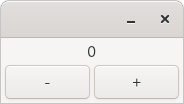
\includegraphics[scale=0.8]{7.png}
    \caption{A simple counting UI}
  \end{figure}

  \begin{lstlisting}[gobble=4,basicstyle=\ttfamily\small]
    module Main (main) where

    import Control.Monad
    import System.Exit
    import qualified Data.Text as Text
    import qualified GI.Gio as G
    import qualified GI.Gtk as Gtk

    main :: IO ()
    main = do
      Just application <- Gtk.applicationNew Nothing [G.ApplicationFlagsDefaultFlags]
      G.onApplicationActivate application (onActivate application)
      status <- G.applicationRun application Nothing
      when (status /= 0) (exitWith (ExitFailure (fromIntegral status)))

    onActivate :: Gtk.IsApplication a => a -> G.ApplicationActivateCallback
    onActivate application = do
      label <- Gtk.labelNew (Just (Text.pack "0"))
      buttonMinus  <- Gtk.buttonNewWithLabel (Text.pack "-")
      buttonPlus <- Gtk.buttonNewWithLabel (Text.pack "+")

      buttonBox <- Gtk.buttonBoxNew Gtk.OrientationHorizontal
      Gtk.boxSetSpacing buttonBox 4
      Gtk.containerAdd buttonBox buttonMinus
      Gtk.containerAdd buttonBox buttonPlus

      box <- Gtk.boxNew Gtk.OrientationVertical 4
      Gtk.widgetSetMarginStart box 4
      Gtk.widgetSetMarginEnd box 4
      Gtk.widgetSetMarginTop box 4
      Gtk.widgetSetMarginBottom box 4
      Gtk.containerAdd box label
      Gtk.containerAdd box buttonBox

      window <- Gtk.applicationWindowNew application
      Gtk.windowSetTitle window Text.empty
      Gtk.windowSetResizable window False
      Gtk.containerAdd window box

      Gtk.onButtonClicked buttonMinus $ do
        t <- Gtk.labelGetLabel label
        Gtk.labelSetLabel label (Text.pack (show (read (Text.unpack t) - 1)))

      Gtk.onButtonClicked buttonPlus $ do
        t <- Gtk.labelGetLabel label
        Gtk.labelSetLabel label (Text.pack (show (read (Text.unpack t) + 1)))

      Gtk.widgetShowAll window
  \end{lstlisting}

  The entry point \lstinline@main@ is just some boilerplate code to invoke a
  callback which starts the actual application. The window and all its contents
  are built in \lstinline@onActivate@.

  The first three lines of \lstinline@onActivate@ create a label initially set
  to \lstinline@0@ and two buttons: \lstinline@buttonMinus@ and
  \lstinline@buttonPlus@. Note that \lstinline@gi-gtk@ employs the
  \lstinline@Text@ data type instead of \lstinline@String@ for efficiency;
  to convert between the two, \lstinline@Text.packpack :: String -> Text@ and
  \lstinline@Text.unpack :: Text -> String@ have to be used.

  To position the two buttons horizontally, a \lstinline@Gtk.ButtonBox@
  container has to be employed. Buttons are added to such container with
  \lstinline@Gtk.containerAdd@; spacing between buttons is configured with
  \lstinline@Gtk.boxSetSpacing@.

  To position the button box below the label created earlier, a
  \lstinline@Gtk.Box@ container is used. Some margin is added on all four sides
  of the container with \lstinline@Gtk.widgetSetMarginStart@,
  \lstinline@Gtk.widgetSetMarginEnd@, \lstinline@Gtk.widgetSetMarginTop@,
  \lstinline@Gtk.widgetSetMarginBottom@.

  The main window is created with \lstinline@Gtk.applicationWindowNew@. Its
  title is set to the empty string and it is configured not to be resizable.
  Finally, event handlers for button clicks are registered with
  \lstinline@Gtk.onButtonClicked@. After all is done, the application window is
  displayed to the user with \lstinline@Gtk.widgetShowAll@.

  As can be seen, using GTK+ within Haskell is not too difficult, even if
  imperative-style programming is required. In most circumstances, code working
  in C has an almost direct relationship with code producing the same result,
  but written in Haskell.

  The package \lstinline@gi-gtk-hs@ provides an idiomatic API on top of
  \lstinline@gi-gtk@ to load widgets from XML strings. The following listing
  illustrates its usage:

  \begin{lstlisting}[gobble=4,basicstyle=\ttfamily\small]
    import qualified Data.GI.Gtk.BuildFn as Gtk

    onActivate' :: Gtk.IsApplication a => a -> G.ApplicationActivateCallback
    onActivate' application = do
      let string =
            "<interface>\n\
            \  <object class=\"GtkApplicationWindow\" id=\"window\">\n\
            \    <property name=\"title\"></property>\n\
            \    <property name=\"resizable\">false</property>\n\
            \    <child>\n\
            \      <object class=\"GtkBox\">\n\
            \        <property name=\"orientation\">vertical</property>\n\
            \        <property name=\"spacing\">4</property>\n\
            \        <property name=\"margin\">4</property>\n\
            \        <child>\n\
            \          <object class=\"GtkLabel\" id=\"label\">\n\
            \            <property name=\"label\">0</property>\n\
            \          </object>\n\
            \        </child>\n\
            \        <child>\n\
            \          <object class=\"GtkButtonBox\">\n\
            \            <property name=\"orientation\">horizontal</property>\n\
            \            <property name=\"spacing\">4</property>\n\
            \            <child>\n\
            \              <object class=\"GtkButton\" id=\"buttonMinus\">\n\
            \                <property name=\"label\">-</property>\n\
            \              </object>\n\
            \            </child>\n\
            \            <child>\n\
            \              <object class=\"GtkButton\" id=\"buttonPlus\">\n\
            \                <property name=\"label\">+</property>\n\
            \              </object>\n\
            \            </child>\n\
            \          </object>\n\
            \        </child>\n\
            \      </object>\n\
            \    </child>\n\
            \  </object>\n\
            \</interface>\0"

      let buildFn = do
            label <- Gtk.getObject Gtk.Label (Text.pack "label")
            buttonMinus <- Gtk.getObject Gtk.Button (Text.pack "buttonMinus")
            buttonPlus <- Gtk.getObject Gtk.Button (Text.pack "buttonPlus")
            window <- Gtk.getObject Gtk.ApplicationWindow (Text.pack "window")

            Gtk.onButtonClicked buttonMinus $ do
              t <- Gtk.labelGetLabel label
              Gtk.labelSetLabel label (Text.pack (show (read (Text.unpack t) - 1)))

            Gtk.onButtonClicked buttonPlus $ do
              t <- Gtk.labelGetLabel label
              Gtk.labelSetLabel label (Text.pack (show (read (Text.unpack t) + 1)))

            pure window

      builder <- Gtk.builderNewFromString (Text.pack string) (-1)
      window <- Gtk.buildWithBuilder buildFn builder
      Gtk.windowSetApplication window (Just application)
      Gtk.widgetShowAll window
  \end{lstlisting}

  \backmatter

  \conclusions

  % TODO

  \appendix

  \chapter{Devin source code}

  \section{\texttt{devin.cabal}}

  \lstinputlisting
    [aboveskip=0pt,basicstyle=\ttfamily\footnotesize]
    {../devin.cabal}

  \section{\texttt{src/Devin/Display.hs}}

  \lstinputlisting
    [aboveskip=0pt,basicstyle=\ttfamily\footnotesize]
    {../src/Devin/Display.hs}

  \section{\texttt{src/Devin/Error.hs}}

  \lstinputlisting
    [aboveskip=0pt,basicstyle=\ttfamily\footnotesize]
    {../src/Devin/Error.hs}

  \section{\texttt{src/Devin/Evaluator.hs}}

  \lstinputlisting
    [aboveskip=0pt,basicstyle=\ttfamily\footnotesize]
    {../src/Devin/Evaluator.hs}

  \section{\texttt{src/Devin/Evaluators.hs}}

  \lstinputlisting
    [aboveskip=0pt,basicstyle=\ttfamily\footnotesize]
    {../src/Devin/Evaluators.hs}

  \section{\texttt{src/Devin/Interval.hs}}

  \lstinputlisting
    [aboveskip=0pt,basicstyle=\ttfamily\footnotesize]
    {../src/Devin/Interval.hs}

  \section{\texttt{src/Devin/Parsec.hs}}

  \lstinputlisting
    [aboveskip=0pt,basicstyle=\ttfamily\footnotesize]
    {../src/Devin/Parsec.hs}

  \section{\texttt{src/Devin/Parsers.hs}}

  \lstinputlisting
    [aboveskip=0pt,basicstyle=\ttfamily\footnotesize]
    {../src/Devin/Parsers.hs}

  \section{\texttt{src/Devin/Syntax.hs}}

  \lstinputlisting
    [aboveskip=0pt,basicstyle=\ttfamily\footnotesize]
    {../src/Devin/Syntax.hs}

  \section{\texttt{src/Devin/Type.hs}}

  \lstinputlisting
    [aboveskip=0pt,basicstyle=\ttfamily\footnotesize]
    {../src/Devin/Type.hs}

  \section{\texttt{src/Devin/Typer.hs}}

  \lstinputlisting
    [aboveskip=0pt,basicstyle=\ttfamily\footnotesize]
    {../src/Devin/Typer.hs}

  \section{\texttt{src/Devin/Typers.hs}}

  \lstinputlisting
    [aboveskip=0pt,basicstyle=\ttfamily\footnotesize]
    {../src/Devin/Typers.hs}

  \section{\texttt{src/Devin/Utils.hs}}

  \lstinputlisting
    [aboveskip=0pt,basicstyle=\ttfamily\footnotesize]
    {../src/Devin/Utils.hs}

  \section{\texttt{test/Main.hs}}

  \lstinputlisting
    [aboveskip=0pt,basicstyle=\ttfamily\footnotesize]
    {../test/Main.hs}

  \section{\texttt{test/Devin/EvaluatorsSpec.hs}}

  \lstinputlisting
    [aboveskip=0pt,basicstyle=\ttfamily\footnotesize]
    {../test/Devin/EvaluatorsSpec.hs}

  \section{\texttt{test/Devin/ParsersSpec.hs}}

  \lstinputlisting
    [aboveskip=0pt,basicstyle=\ttfamily\footnotesize]
    {../test/Devin/ParsersSpec.hs}

  \section{\texttt{test/Devin/TypersSpec.hs}}

  \lstinputlisting
    [aboveskip=0pt,basicstyle=\ttfamily\footnotesize]
    {../test/Devin/TypersSpec.hs}

  \section{\texttt{app/Main.hs}}
  \label{section:appmain}

  \lstinputlisting
    [aboveskip=0pt,basicstyle=\ttfamily\footnotesize]
    {../app/Main.hs}

  \section{\texttt{app/Devin/Highlight.hs}}

  \lstinputlisting
    [aboveskip=0pt,basicstyle=\ttfamily\footnotesize]
    {../app/Devin/Highlight.hs}

  \section{\texttt{app/Devin/Tree.hs}}

  \lstinputlisting
    [aboveskip=0pt,basicstyle=\ttfamily\footnotesize]
    {../app/Devin/Tree.hs}

  \section{\texttt{app/Devin/Highlight/Braces.hs}}

  \lstinputlisting
    [aboveskip=0pt,basicstyle=\ttfamily\footnotesize]
    {../app/Devin/Highlight/Braces.hs}

  \section{\texttt{app/Devin/Highlight/Syntax.hs}}

  \lstinputlisting
    [aboveskip=0pt,basicstyle=\ttfamily\footnotesize]
    {../app/Devin/Highlight/Syntax.hs}

  \printbibliography
\end{document}
